\documentclass[runningheads]{llncs}
\newcommand\numberthis{\addtocounter{equation}{1}\tag{\theequation}} % numbering equations

\usepackage{cite}
\usepackage[utf8]{inputenc}
\usepackage{graphicx}
\usepackage{amsmath}
\usepackage{amsfonts}
\usepackage{color}
\usepackage{amssymb}
\usepackage{mathtools}
\usepackage{float}
\usepackage{multirow}
\usepackage{caption}
\usepackage{algorithm2e}


\RestyleAlgo{boxruled}




%% Sets
\newcommand{\cnums}{\mathbb{C}} % complex numbers
\newcommand{\reals}{\mathbb{R}}
\newcommand{\rationals}{\mathbb{Q}}
\newcommand{\integers}{\mathbb{Z}} % integers
\newcommand{\double}{\mathbb{D}} % double precision floating point numbers
\newcommand{\intervals}{\mathbb{I}} % set of intervals with bounds in double and ${-\infty,\infty}$
\newcommand{\set}[1]{\left\{#1\right\}} % set
\newcommand{\st}[1]{\left|~#1\right.} % such that
\newcommand{\fe}[1]{ \mathbb{F}_{#1} } % mathematical expressions
\newcommand{\vars}{V} % variables
\newcommand{\ball}[2]{\mathbb{B}\rb{#1,#2}} % open box with a radius
\newcommand{\interval}[2]{\sqb{#1,#2}} % interval
\newcommand{\dom}[1]{\operatorname{Dom}\rb{#1}} % domain of a function expression

%% Braces
\newcommand{\rb}[1]{\left(#1\right)}
\newcommand{\sqb}[1]{\left[#1\right]}

%% Linear algebra
\newcommand{\mymatrix}[1]{\begin{bmatrix}#1\end{bmatrix}} % matrix
\newcommand{\identity}[1]{\mathcal{I}_{#1}} % identity matrix
\newcommand{\rows}[1]{\operatorname{rows}\left(#1\right)} % number of rows in a matrix
\newcommand{\cols}[1]{\operatorname{cols}\left(#1\right)} % number of columns in a matrix
\newcommand{\diag}[1]{\mathcal{D}\rb{#1}} % diagonal matrix

%% Operators
\newcommand{\abs}[1]{\left|#1\right|} % absolute value
\newcommand{\minsum}{\oplus}
\newcommand{\norm}[1]{\left\|#1\right\|}
\newcommand{\meet}[2]{#1\bigwedge #2} % Meet
\newcommand{\join}[2]{#1\bigvee #2} % Join
\newcommand{\conv}[1]{\operatorname{{Conv}}\rb{#1}}
\newcommand{\real}[1]{\operatorname{Re}\rb{#1}}  % real part
\newcommand{\imag}[1]{\operatorname{Im}\rb{#1}}  % imaginary part
\DeclareMathOperator*{\argmin}{arg\,min} % arg min
\newcommand{\card}[1]{\#{#1}}

%% notes
\newcommand{\todo}[1]{todo: {\color{red}#1}}

%----------------------------------------------------------------------
%% paper specific
%----------------------------------------------------------------------
%% sets
\newcommand{\init}{\Psi}  % initial set
\newcommand{\inpset}{{U}} % input set

%% symbols
\newcommand{\proj}[1]{\lambda_{#1}} % function symbol for projection on a dimension
\newcommand{\trfn}[1]{\mathbf{#1}} % trajectory function
\newcommand{\gen}{G} % generator
\newcommand{\cen}{c} % center
\newcommand{\bounds}{d} % bounds
\newcommand{\eig}{\Lambda}  % eigenvectors at origin
\newcommand{\zt}{Z} % zonotope tuple

%% functions
\newcommand{\grad}[1]{\nabla{#1}} % gradient
\newcommand{\hess}[1]{\operatorname{H}{#1}} % hessian
\newcommand{\iv}[2]{\mu\rb{#1}\rb{#2}} % interval bounds on a function expression
\newcommand{\ivmat}[1]{\mu\rb{#1}} % interval matrix converted from double
\newcommand{\tr}[2]{\mathbf{#1}\rb{#2}} % trajectory value
\newcommand{\reach}[3]{\mathbf{#1}_{#2}\rb{#3}} % reachable set
\newcommand{\taylor}[3]{\sigma\rb{#1,#2,#3}} % taylor error
\newcommand{\mi}[1]{\alpha\rb{#1}} % center of an interval matrix
\newcommand{\rad}[1]{\beta\rb{#1}} % error of an interval matrix
\newcommand{\stmat}[3]{\mathcal{A}_{#1}^{#2,#3}} % state action matrix
\newcommand{\inpmat}[3]{\mathcal{B}_{#1}^{#2,#3}} % input action matrix
\newcommand{\err}[3]{E_{#1,#2,#3}} % additive remainder term in linearization
\newcommand{\dismat}[3]{{#1}^{#2}_{#3}} % discrete time action matrix
\newcommand{\iz}[3]{\left\llbracket\rb{#1,#2,#3}\right\rrbracket} % interval zonotope
\newcommand{\lin}[3]{\mathcal{T}\rb{#1,#2,#3}} % interval zonotope
\newcommand{\ivflow}[5]{\mathcal{S}_{#1,#2}^{#3,#4}\rb{#5}} % flow approximation inside an interval
\newcommand{\flow}[5]{\mathcal{R}_{#1,#2}^{#3,#4}\rb{#5}} % flow approximation at a time point
\newcommand{\utaylor}[4]{\widehat{\sigma}\rb{#1,#2,#3,#4}} % upper bound on taylor error
\newcommand{\dopt}[1]{O\rb{#1}} % optimum division vector
\newcommand{\iouopt}[2]{P^{#1}\rb{#2}} % optimum iou of interval zonotopes
\DeclareMathOperator*{\refine}{\pi} % refine
\newcommand{\ztset}[1]{\left\llbracket{#1}\right\rrbracket}
\newcommand{\zerozon}[2]{\zt_{#1\times #2}\rb{0}}


\title{Intersection of Unions Flowpipe for Minimizing Multi-Directional Linearization Error}
\titlerunning{Intersection of Unions Flowpipe for Minimizing Multi-Directional}
\author{}
\institute{}
%
\begin{document}    
\maketitle
%
\begin{abstract}
We propose a new efficient method for computing an overapproximation
of a set of trajectories, called flowpipe, for a system
described by uncertain nonlinear differential equations.  Since
reachable sets of linear systems can be computed efficiently,
piecewise linearization of nonlinear ODEs is a commonly used technique
while computing flowpipes.  However, the number of pieces required in
piecewise linearization becomes exponential in the dimension for
minimizing the linearization error below any threshold value, which
can be computationally intractable in high dimensions.  Alternatively,
if the number of divisions is fixed, we need to optimize the way the
reach set is divided to minimize the linearization error.  Since the
linearization error is multi-dimensional, this minimization is a
multi-objective optimization problem that does not have a single best
solution.  However, a previous method in literature proposed to
minimize a single dimensional measure while dividing the reachable
sets, which does not necessarily reduce the linearization error along
all coordinates.  In this paper, we propose a better method where we
use multiple best optimal ways of division, instead of a single way of
division, for minimizing linearization error along multiple
directions.  Consequently, we represent the resulting reachable sets
as the intersection of unions (IoU), where each intersecting union
corresponds to the optimized division for each direction among
multiple directions.  We propose an algorithm to propagate the
resulting IoU of sets such that the linearization error is reduced
significantly along every direction in a set of multiple directions.
As a proof of concept, we evaluate our algorithm on an illustrative
example and two high dimensional real-world examples and demonstrate a
high increase in the flowpipe accuracy compared to the earlier method
of division and other state-of-the-art methods.
\end{abstract}

\section{Introduction}
The dynamics of many real world systems is modeled by ordinary
differential equations (ODEs).  These models typically contain
uncertainties in the parameters, inputs and initial conditions to
account for the unpredictable behavior of the system.  To ensure
reliable behavior of the systems, especially those which are safety
critical, these ODE models have to be verified to satisfy the
requirements for the correct operation of the system.  Verifying
properties of the ODE models (eg. safety, stability) requires
approximating the set of trajectories (solutions) of the ODE in the
presence of uncertainties.  But exactly computing the set of
trajectories of nonlinear ODEs can be computationally intractable,
because computing accurate images of nonlinear maps is at least NP
Hard~\cite{murty1985some}.  Alternatively, significant research has
been carried out on overapproximating the set of trajectories of
nonlinear uncertain ODEs by data
structures~\cite{chen2012taylor,testylier2013nltoolbox,althoff2013reachability,kochdumper2020sparse,ramdani2009hybrid,han2006reachability,maidens2014reachability},
referred to as \emph{flowpipes}~\cite{chen2012taylor}.

Nevertheless, computing accurate images of nonlinear multivariable
functions is at least NP Hard~\cite{murty1985some}.  Therefore, the
computational complexity of any flowpipe computation algorithm for
nonlinear systems can blow up beyond tractable limits while ensuring a
desired accuracy in high dimensions.  For instance, a commonly used
method in flowpipe computation is piecewise
linearization~\cite{ramdani2009hybrid,han2006reachability,althoff2008reachability,li2020reachability,dang2010accurate,bak2016scalable},
where the nonlinear ODEs are approximated by piecewise linear ODEs.
The advantage of piecewise linearization is that reachable sets of
linear ODEs can be computed far more efficiently than nonlinear ODEs.
However, the number of pieces required to ensure that the
linearization error is below a threshold increases exponentially in
the dimension of ODEs.  To our understanding, no effective solution
has yet been proposed to tackle the \emph{curse of dimensionality} in
piecewise linearization based flowpipe computation.  Some techniques
attempt to decompose the nonlinear system in higher dimensions into
subsystems with lower
dimensions~\cite{chen2018decomposition,chen2016decomposed}.  However,
the decomposition of nonlinear dynamics only scales effectively when
there exist small dimensional subsystems with loose coupling, but not
otherwise.

Alternatively, to avoid blowing up the number of pieces in piecewise
linearization, we can fix the number of pieces.  Then, we need to
optimize the way the reachable set is divided into subsets to minimize
the linearization error.  In this regard, prior work has been done by
Althoff. et. al.~\cite{althoff2008reachability} to optimally split
reachable sets for minimizing the linearization error.  They use a
single dimensional measure of reduction in linearization error while
splitting a reachable set.  However, the linearization error is a
multi-dimensional vector for which there is no single best optimum way
of splitting.  For different directions, there are different optimal
ways of splitting the reachable set.  Therefore, this splitting method
based on optimizing a single dimensional measure may not provide
desired accuracy along all coordinates.  This drawback is explained in
Section~\ref{sec:motivation} of our paper with an illustrative
example.

In this paper, we propose a more efficient way of minimizing the
multi-dimensional linearization error in flowpipe computation.  We use
different optimal divisions of a reachable set for minimizing the
linearization error along different directions, instead of a one way
of dividing the set.  Consequently, our reachable set is represented
as an intersection of the unions (IoU) of sets resulting from
different optimal ways of dividing the set, for different directions
of linearization error.  Then the linearization error is effectively
reduced along all directions in a given finite set of multiple
directions.  We develop an algorithm to propagate the intersection of
unions reachable set for flowpipe computation.  As a proof-of-concept,
we evaluate our algorithm on an illustrative example and two high
dimensional real-world examples. Our IoU flowpipe method showed a high
increase in the flowpipe accuracy compared to the earlier method of
division~~\cite{althoff2008reachability} and other state-of-the-art
methods~\cite{chen2012taylor,althoff2013reachability}.

In summary, we make the following contributions in this paper.
\begin{enumerate}
\item We introduce the use of intersection of unions, instead of
    just union, to minimize linearization error along multiple
    directions during flowpipe computation.  The use of intersection
    of union of sets is novel and has not been employed in previous
    research.
%
\item We develop a parallel algorithm to propagate IoU reachable sets
    over time.  The algorithm uses a variant of zonotope,
    called \emph{interval zonotope}, for computing intersection
    between zonotopes fastly and more accurately than simple zonotopes.
%
\item We demonstrate high increase in flowpipe accuracy on two high
    dimensional real world examples, compared to other state-of-the
    art methods.  Also, the computation time of our parallel
    algorithm is comparable or better than other approaches on
    multi-core machines.
\end{enumerate}
%
The comparison with related work is done in Section~\ref{sec:related}.

%
\section{Preliminaries}
\subsection{Notation}
The set of real numbers is $\reals$, integers is $\integers$, and
complex numbers is $\cnums$.  The subset of real numbers that can be
represented in double precision floating point format is $\double$.
For $\Psi\subseteq\reals$, $a\in\reals$ and
$\bowtie\in\set{\geq,\leq,>,<}$, we denote $\Psi_{\bowtie a} = \set{
  x\in\Psi \st x \bowtie a }$.  For example, $\double_{>3.2} =
\set{x\in\double\st{x>3.2}}$.  The supremum of a subset of real numbers
$\Psi\subseteq\reals$ is $\sup\rb{\Psi}\in\reals\bigcup\set{\infty}$
and the infimum is $\inf\rb{\Psi}\in\reals\bigcup\set{-\infty}$.  The
absolute value of a real number $x$ is $\abs{x} = \sup\set{x,-x}$.
The real part of a complex number $z$ is $\real{z}$ and the imaginary
part is $\imag{z}$.  The absolute value of a complex number $z$ is
$\abs{z} = \rb{(\real{z})^2 + (\imag{z})^2}^{1/2}$.  For two reals $r$
and $s$, the result of multiplying $r$ and $s$ is $rs$, the result of
adding of $r$ and $s$ is $r+s$, the result of subtracting $s$ from $r$
is $r-s$ and the result of dividing $r$ by $s$ if $s\neq 0$ is
$\frac{r}{s}$.  For non-negative integer $i$ and real number $x$, the
result of raising $x$ to the power $i$ is $x^i$.  The set of $n\times
m$ matrices containing elements from a set $\Psi$ is $\Psi^{n\times
  m}$.  For simplicity, we denote $\Psi^{n\times 1}$ as $\Psi^n$.  The
set of real vectors is $\reals^n$.  The $i^{th}$ row $j^{th}$ column
element of a matrix $X$ is denoted $X_{ij}$.  Similarly, for real
vector $x$, $x_i$ denotes the $i^{th}$ component of $x$.  The
submatrix of $X$ containing rows $l_1$ to $l_2$ and columns $k_1$ to
$k_2$ is denoted by $X_{l_1:l_2,k_1:k_2}$.  An $n\times m$ matrix
containing a repeated element $z$ is denoted $\sqb{z}_{n\times m}$.
The identity $n\times n$ square matrix containing all ones along its
diagonal and rest zeros is denoted $\identity{n}$.  The transpose of a
matrix $X$ is $X^T$ where $X^T_{ij} = X_{ji}$.  For
$X\in\reals^{n\times m}$ and $Y\in\reals^{m\times p}$, the matrix
product is $XY\in\reals^{n\times p}$ where $\forall
i\in\set{1,\ldots,n},\forall j\in\set{1,\ldots,p},\rb{XY}_{ij} =
\sum_{k=1}^{m}X_{ik}Y_{kj}$.  The euclidean norm of a real vector
$x\in\reals^n$ is $\norm{x} = \rb{\sum_{i=1}^n\abs{x_i}^2}^{1/2}$.
The infinity norm is $\norm{x}_\infty =
\sup\set{\abs{x_1},...,\abs{x_n}}$.  For $r\in\reals_{> 0}$ and
$x\in\reals^n$, we define the box of width $r$ around $x$ as
$\ball{x}{r} = \set{ y\in\reals^n: \norm{y - x}_\infty \leq r }$.

If $\Psi\subseteq\reals^n$, a function $f:\Psi\rightarrow\reals^m$ is
called \emph{continuous} if $\forall
x\in\Psi,\forall\epsilon\in\reals_{>0}$, there exists
$\delta\in\reals^n$ such that if $y\in\ball{x}{\delta}\bigcap\Psi$,
then $f(y)\in\ball{f(x)}{\epsilon}$.  A function
$f:\Psi\rightarrow\reals^m$ is called \emph{piecewise continuous} if
there exists a finite number of sets $\Psi_1,\ldots,\Psi_k$ such that
$\bigcup_{i=1}^k\Psi_i=\Psi$ and $f_i:\Psi_i\rightarrow
\reals^m$ where $\forall x\in\Psi_i~f_i\rb{x}=f\rb{x}$, is continuous
for all $i\in\set{1,\ldots,k}$.

A partial function $f:\reals^n\rightarrow \reals^m$ is a relation $f
\subseteq\reals^n\times\reals^m$ such that if $(x,y_1),(x,y_2)\in
f$, then $y_1=y_2 = f(x)$.  The domain of a partial function
$f:\reals^n\rightarrow\reals^m$ is $\dom{f}
= \set{x\in\reals^n\st{\exists y\in\reals^m,~(x,y)\in f}}$.  Given two
partial functions $f:\reals^n\rightarrow\reals^m$ and
$g:\reals^m\rightarrow\reals^p$, their composition is $f\circ g
= \set{(x,y)\in\reals^{n\times p} \is{This \ has \ to \ be \reals^{n}\times \reals^p?}} \st{\exists z\in\reals^m~(x,z)\in
f,~(z,y)\in g}}$.  For every $n\in\integers_{>0}$, we consider the
subset $\fe{n}$ of partial functions, defined recursively as follows.
%
\begin{enumerate}
\item $f\in\fe{n}$ if $\exists a\in\double^n,f = \set{(x,a^Tx)\st{x\in\reals^n}}$. 
\item $\forall f_1,f_2\in\fe{n}, \set{ \frac{1}{f_1}, f_1+f_2, f_1-f_2, f_1f_2}\subseteq\fe{n}$.
\item $\forall f\in\fe{n}, \set{ \sin\circ{f}, \cos\circ{f}, \exp\circ{f}, \log\circ{f} } \subseteq \fe{n}$. 
\end{enumerate}
%
We say that the \emph{symbolic derivative} of
$f\in\fe{n}$ exists and is equal to a tuple of partial functions $\nabla f = \rb{\nabla_1
f,\ldots,\nabla_n f}\in\fe{n}^n$ if all of the following are true.
%
\begin{itemize}
\item $\forall i\in\set{1,\ldots,n}$, $\dom{f}\subseteq \dom{\nabla_i f}$.
\item $\forall x\in\dom{f}$ and $\forall\epsilon\in\reals_{>0}$, there exists $r\in\reals_{>0}$ 
such that $\forall h\in\ball{0}{r}$, we have $(x+h)\in\dom{f}$ and
%
\begin{align*}
& \frac{\norm{f\rb{x+h}-\sum_{i=1}^n \nabla_if\rb{x}h_i}}{\norm{h}}
< \epsilon.~\numberthis\label{eqn:symder}
\end{align*}
%
\end{itemize}
%
\begin{example}
Let us consider a partial function $f\in\fe{2}: f(x,y) =
\frac{sin\rb{y}}{x}$.  By applying the basic rules of calculus, we get
$\frac{\partial{f}}{\partial{x}}\left|_{x,y}\right. =
\frac{-sin(y)}{x^2}$ and
$\frac{\partial{f}}{\partial{y}}\left|_{x,y}\right. =
\frac{\rb{cos(y)}}{x}$. So, the pair of partial functions $\rb{
  \rb{(x,y),\frac{-sin(y)}{x^2}}, \rb{(x,y), \frac{{cos(y)}}{x}} }$
  is a symbolic derivative of $f$.  
\end{example}
%
\emph{Remark:}  For the specific subset of partial functions $\fe{n}$
  defined above,
  if $f\in\fe{n}$, the symbolic derivative $\nabla{f}$ and the
symbolic double derivative $\nabla^2f\in\fe{n}^{n\times
n}: \rb{\nabla^2 f}_{ij} =
\nabla_j\nabla_i f$ exist.  They can be computed by using
basic rules of calculus.
%
\subsection{Use of interval arithmetic}
For $a,b\in\double$ such that $a<b$, we denote\\ $\interval{a}{b} =
\set{x\in\reals\st a\leq x\leq b}$, $[-\infty,a] = \set{x\in\reals\st
  x\leq a}$, $[a,\infty) = \set{x\in\reals\st a\leq x}$ and
  $[-\infty,\infty] = \reals$.  We denote the set of all intervals as
  $\intervals$.  For $u,v\in\intervals$, interval arithmetic
  (see~\cite{bronnimann2006design}) gives us interval bounds
  $uv,(u+v),(u-v)\in\intervals$ such that $uv\supseteq\set{xy\st x\in
    u, y\in v}$, $\rb{u+v}\supseteq\set{x+y\st x\in u, y\in v}$ and
  $\rb{u-v}\supseteq\set{x-y\st x\in u, y\in v}$.  Similarly, for a
  partial function $f\in \fe{n}$ and interval $u\in\dom{f}$, we use
  interval arithmetic to correctly bound the image of $f$ over $a$,
  denoted $\iv{f}{u} \supseteq \set{f\rb{x}\st{x\in u} }$.


The set of $n\times m$ interval matrices is $\intervals^{n\times m}$,
and $n$-dimensional interval vectors is $\intervals^{n\times 1}$,
conveniently denoted by $\intervals^{n}$.  For $A\in\reals^{n\times
m}$ and $\bar{X}\in\intervals^{n\times m}$, we say $A\in \bar{X}$ if
$\forall
\rb{i,j}\in\set{1,\ldots,n}^2, A_{ij}\subseteq \bar{X}_{ij}$.  The interval
matrix $X$ is said to be bounded if $\forall
i\in\set{1,\ldots,n}, \forall j\in\set{1,\ldots,m}, \exists
a,b\in\double: \bar{X}_{ij} = [a,b]$.  The matrix product
$\bar{X}\bar{Y}$ of two interval matrices
$\bar{X}\in\intervals^{n\times p}$ and $\bar{Y}\in\intervals^{p\times
m}$ is $\bar{X}\bar{Y} = \sum_{k=1}^p\bar{X}_{ik}\bar{Y}_{kj}$. The
sum of interval matrices $\bar{X}$ and $\bar{Y}$ is $\bar{X}
+ \bar{Y}$, where $\rb{\bar{X}+\bar{Y}}_{ij} = \bar{X}_{ij}
+ \bar{Y}_{ij}$.  It follows that if $A\in \bar{X}$ and
$B\in \bar{Y}$, then $AB\in \bar{X}\bar{Y}$ and
$A+B\in \bar{X}+\bar{Y}$.  If $X\in\double^{n\times m}$, then
$\ivmat{X}\in\intervals$ is an interval matrix such that $\forall
(i,j)\in\set{1,\ldots,n}\times\set{1,\ldots,m}, \ivmat{X}_{ij} =
[X_{ij},X_{ij}]$.  For an interval matrix $\bar{X}$, we denote $\mi{\bar{X}} =
\frac{\ivmat{\sup\rb{\bar{X}}} + \ivmat{\inf\rb{\bar{X}}}}{[2,2]}$ and $\rad{X} =
\bar{X} - \mi{\bar{X}}$.  The diagonal interval matrix containing elements of an
interval vector $u$ along its diagonal is denoted $\diag{u}$.  If
$f\in\fe{n}^{m\times p}$ is a matrix of function expressions, then
$\iv{f}{u}\in \intervals^{m\times p}$ is an interval matrix where
$\rb{\iv{f}{u}}_{ij} = \iv{f_{ij}}{u}$.  For $u,v\in\intervals$, we
denote $\meet{u}{v} =
[\sup\rb{\inf\rb{u},\inf\rb{v}},\inf\rb{\sup\rb{u},\sup\rb{v}}]$ and
$\join{u}{v} = [\inf\rb{u\bigcup v}, \sup\rb{u\bigcup v}]$.  If
$\bar{X},\bar{Y}\in\intervals^{n\times m}$, then
$\meet{\bar{X}}{\bar{Y}},\join{\bar{X}}{\bar{Y}}\in\intervals^{n\times m}$ such that
$\rb{\meet{\bar{X}}{\bar{Y}}}_{ij} = \meet{\bar{X}_{ij}}{\bar{Y}_{ij}}$ and
$\rb{\join{\bar{X}}{\bar{Y}}}_{ij} = \join{\bar{X}_{ij}}{\bar{Y}_{ij}}$.
%
In addition to the above intervals, we denote
%
$[a,b) = \set{x\in\reals\st{a\leq x<b}}$, $(a,b] = \set{x\in\reals\st{a< x\leq b}}$, $(a,b) = \set{x\in\reals\st{a< x < b}}$.


%\subsection{Nonlinear system and linearization}
%An $n$-dimensional nonlinear dynamical system with $m$ inputs is
specified by a tuple $\rb{f,\inpset,\Omega}$ where $f =
\rb{f_1,\ldots,f_n}\in \fe{n+m}^n$ is an
$n$-tuple of partial functions in $\fe{n+m}^n$, an interval vector
$\inpset\in\intervals^m$ is called the \emph{input set} and
$\Omega\in\intervals^n$ is called the \emph{state space}.  For any
$T\in\reals_{>0}$, a function $\trfn{x}:[0,T)\rightarrow \reals^n$ is
called a \emph{state trajectory} if there exists a \emph{piecewise
continuous} function $\trfn{u}:[0,T)\rightarrow \inpset$,
called \emph{input trajectory}, such that all of the following is
true.
%
\begin{align*}
& \forall t\in[0,T), \tr{x}{t}\subseteq \Omega,\\
& \forall
t\in[0,T)\forall\epsilon\in\reals_{>0}, \exists\delta\in\reals_{>0}~\text{such
that}\\
& \forall h\in[-\delta,\delta]\bigcap[0,T]~\norm{ \frac{ \tr{x}{t+h}
- \tr{x}{t} }{h} - f_i\rb{ \mymatrix{ \tr{x}{t}\\ \tr{u}{t} }
}}< \epsilon~\numberthis\label{eqn:dynamics}
\end{align*}
%
In rest of the paper, $n$ denotes the dimension of a nonlinear system
and $m$ denotes the number of inputs, unless otherwise stated.  For a
trajectory $\trfn{x}:[0,T)\rightarrow \reals^n$ and $\tau<T$, we
denote $\trfn{x}|_{[0,\tau]}
= \trfn{y}:[0,T)\rightarrow \reals^n: \forall t\in[0,\tau)\tr{y}{t}
= \tr{x}{t}$.
%
Our objective is to compute an overapproximation of the set of all
state trajectories of a nonlinear system.
%
\begin{example}\label{eg:ill}
Let us denote the function expressions $\proj{1} = x$, $\proj{2} = y$,
$\proj{3} = \theta$ and $\proj{4} = u$.  A $3$-dimensional nonlinear
system with one input, state space $\reals^n$ and input set $U =
[-0.3,0.3]$ can be specified as $H = \rb{f,[-0.3,0.3],\reals^3}$ where
%
\begin{align*}
& f_1 = \rb{ u\rb{ x + \theta + 0.1y } - 1}x,
& f_2 = \rb{ u\rb{ y + \theta + 0.1x } - 1}y,\\
& f_3 = -\theta + 0.001\theta^2.
\end{align*}
%
Let us consider the zero input trajectory $\tr{u}{t} = 0~\forall
t\in[0,5)$.  In this case, two state trajectories are $\forall
t\in[0,5)$,
%
\begin{align*}
\tr{x}{t} = \mymatrix{ -0.1\exp\rb{-t}\\ 0.1\exp\rb{-t}\\ 0.1\exp\rb{-t} },~
& \tr{x}{t} = \mymatrix{ -0.2\exp\rb{-t}\\ -0.1\exp\rb{-t}\\ -0.1\exp\rb{-t} }
\end{align*}
%
which begin at $\tr{x}{0} = \mymatrix{-0.1,0.1,0.1}^T$ and $\tr{x}{0}
= \mymatrix{-0.2,-0.3,-0.1}^T$, respectively.
%
There are also state trajectories without an analytic form.
\end{example}
%
%% The \emph{reachable set} of the nonlinear system $H
%% =\rb{f,\inpset,\Omega}$ from an initial set $\init$ at a time point
%% $t$, denoted $\reach{H}{t}{\init}$, is a set containing all points
%% $\tr{x}{t}$ where $\trfn{x}$ is a state trajectory of $H$ and
%% $\tr{x}{0}\in\init$.  Similarly, $\reach{H}{[t_1,t_2]}{\init}
%% = \bigcup_{t\in[t_1,t_2]}\reach{H}{t}{\init}$.  Computing the exact
%% reachable set of nonlinear systems is computationally infeasible in
%% general because nonlinear ODEs may not have analytically closed form
%% solutions.  Instead, an overapproximation of the reachable set at each
%% time point, called \emph{flowpipe}, can be computed to verify
%% essential reachability properties like safety and stability.  The
%% flowpipe approximation of reachable set is
%% represented in a computer by a data structure which can be manipulated
%% efficiently to check reachability properties.  Such data structures
%% are called set representations, whose examples
%% are \emph{boxes}, \emph{polytopes}, \emph{zonotopes}, \emph{Taylor
%% models}, \emph{barrier certificates} and \emph{polynomial
%% zonotopes}~(\todo{cite all}).
%
\paragraph{Linearization:}  We say that a dynamical system
$L = \rb{g,U\times V,\Omega}$ where $g\in\fe{2n+m}^n$ is
linear if we have matrices $A\in\reals^{n\times n}$ and
$B\in\reals^{m\times n}$ such that forall $i\in\set{1,\ldots,n}$,
$x\in\reals^n$, $u\in U$ and $v\in V$, we have
%
\begin{align*}
& g_i\rb{\mymatrix{x^T & u^T & v^T}^T} = \rb{Ax + Bu + v}_i.
\end{align*}
%
For convenience, we also denote the above linear system as $L
= \rb{A,B,U,V,\Omega}$.  This linear system is said to overapproximate
a nonlinear system $H = \rb{f,\inpset,\Omega}$, denoted $L\succeq H$,
if for all $x\in\Omega$ and $u\in\inpset$, we have $f\rb{\mymatrix{x^T
& u^T}}^T - Ax - Bu \in V$.  In this case, the reachable set of $H$ is
a subset of the reachable set of $L$ at every time point as explained
in the following lemma.
%
\begin{lemma}\label{lem:inclin}
Let us consider that a linear system $L = \rb{A,B,U,V,\Omega}$ is an
overapproximation of a nonlinear system $H = \rb{f,U,\Omega}$.  Then
for all $t\in[0,\infty]$ and $\init\subseteq\Omega$, we have
$\reach{H}{t}{\init}\subseteq \reach{L}{t}{\init}$.
\end{lemma}
%
\begin{proof}
Let us consider a trajectory $\trfn{x}:[0,T)\rightarrow\Omega$ of the
nonlinear system $H$.  Then there exists an input trajectory
$\trfn{u}:[0,T)\rightarrow\Omega$ of $H$ such
that~(\ref{eqn:dynamics}) is true.  Let us define
$\trfn{v}:[0,T)\rightarrow \reals^n$ as $\tr{v}{t} =
f\rb{\mymatrix{\tr{x}{t}^T & \tr{u}{t}^T}}^T - A\tr{x}{t} -
B\tr{u}{t}$.  Since $L$ is an overapproximation of $H$, we have
$\forall t\in[0,T)$, $\tr{v}{t}\in V$.  Then by using
from~(\ref{eqn:dynamics}), for all $\forall t\in[0,T)\epsilon\in\reals_{>0}$, there
exists $\delta\in\reals_{>0}$ such that $\forall
h\in[-\delta,\delta]\bigcap [0,T)$,
%
\begin{align*}
& \norm{ \frac{ \tr{x}{t+h} - \tr{x}{t} }{h} -
f_i\rb{ \mymatrix{ \tr{x}{t}^T & \tr{u}{t}^T }^T }}\\
& = \norm{ \frac{ \tr{x}{t+h} - \tr{x}{t} }{h} -
\rb{A\tr{x}{t} + B\tr{u}{t} + \tr{v}{t}} } < \delta.
\end{align*}
%
Therefore, $\tr{x}{t}$ is also a state trajectory of the linear system
$L$.  So, it follows that
$\reach{H}{t}{\init}\subseteq \reach{L}{t}{\init}$ for all
$\init\subseteq \Omega$.
\end{proof}
%
There are efficient algorithms to compute flowpipes of linear systems
with good accuracy~\cite{girard2005reachability,girard2008efficient}.
So, it would be useful to overapproximate a nonlinear system by a
linear system while computing flowpipe, as follows.
%
\begin{lemma}[Linear overapproximation]\label{lem:linearization}
Let us consider a bounded interval vector $\Omega\in\intervals$, a
vector $c\in\double^n$ and a nonlinear system $H = \rb{f,U,\Omega}$
where $f\in\fe{n+m}^n$ and $U\in\intervals^m$ is a bounded interval
vector.  Let us define $W = \mymatrix{\Omega^T & U^T}^T$,
\begin{align*}
\begin{split}
\stmat{f}{c}{U} = { \iv{{\nabla{f}_{1:n,1:n}}}{ \mymatrix{ \ivmat{c}\\ \mi{U} } } },
%
~\inpmat{f}{c}{U}
= { \iv{{\nabla{f}_{1:n,n+1:n+m}}}{ \mymatrix{ \ivmat{c}\\ \mi{U}}} },
\end{split}\\
%
\begin{split}
& \rb{\taylor{f}{\Omega}{U}}_i
= \frac{1}{2}\sum_{k=1}^{n+m}\sum_{j=1}^{n+m}\iv{\nabla_k\nabla_j{f_i}}{{W}}\rad{W_k}\rad{W_j},~\%
\text{Taylor error}\\
%
& \gamma\rb{f,\Omega,U} = 2\rad{ \stmat{f}{c}{U}\Omega +
\inpmat{f}{c}{U}U
},~~~\%\text{Floating point error bounds}
\end{split}\\
%
\begin{split}
\err{f}{\Omega}{U} = \iv{f}{ \mymatrix{ \ivmat{c}\\ \mi{U} } }
+ \taylor{f}{\Omega}{U} + \gamma\rb{f,\Omega,U}
- \stmat{f}{c}{U}\ivmat{c} - \inpmat{f}{c}{U}\mi{U}.
\end{split}~\numberthis\label{eqn:linearize}
\end{align*}
Then $
H \preceq
\rb{\inf\rb{\stmat{f}{c}{U}},
\inf\rb{\inpmat{f}{c}{U}},
U,
\err{f}{\Omega}{U}
} $
%
\end{lemma}
%
\begin{proof}
Based on Taylor remainder theorem, for all $i\in\set{1,\ldots,n}$
and $z\in W$, there exists $r\in W$ such that
%
\begin{align*}
f_i\rb{z} = & f_i\rb{\mymatrix{\ivmat{c} \\ \mi{U}}} + \nabla
f_i\rb{\mymatrix{\ivmat{c} \\ \mi{U}}}\rb{z - \mymatrix{\ivmat{c} \\ \mi{U}}} +\\
& \frac{1}{2}\sum_{k=1}^{n+m}\sum_{j=1}^{n+m}\rb{\nabla_k\nabla_j{f_i}\rb{r}}\rb{z-\mymatrix{\ivmat{c} \\ \mi{U}}}_j\rb{z-\mymatrix{\ivmat{c} \\ \mi{U}}}_k~\numberthis\label{eqn:taylor}
\end{align*}
%
The lemma follows by substituting both $r$ and $z$ by
the interval vector $W$ in the R.H.S of Equation~(\ref{eqn:taylor}) and applying
interval arithmetic.
\end{proof}
%
\begin{example}
Let us consider the nonlinear system $H = \rb{f,[-0.2,0.2],[-1,1]^3}$
where $f$ is the tuple specified in Example~\ref{eg:ill}.  By applying
Lemma~\ref{lem:linearization}, we get a linear overapproximation $L
= \rb{A,B,[-0.2,0.2],V,[-1,1]^3}\succeq H$ where we illustrate below
how $A_{11}$, $B_{11}$, and $V_{1}$ are computed.
%
\begin{align*}
& A_{11} = \inf\rb{\rb{\frac{df_1}{dx}}\mid_{\rb{x,y,z,u} =
\ivmat{(0,0,0,0)}}} \\ & = \inf\rb{\rb{u\rb{ x + \theta + 0.1y } - 1 +
xu}\mid_{\rb{x,y,z,u} = \ivmat{(0,0,0,0)}}} = -1 \\
%
& B_{11} = \inf\rb{\rb{\frac{df_1}{du}}\mid_{\rb{x,y,z,u} =
\ivmat{(0,0,0,0)}}} \\ &= \inf\rb{\rb{x\rb{ x + \theta + 0.1y
}}\mid_{\rb{x,y,z,u} = \ivmat{(0,0,0,0)}}} = 0 \\
%
& \nabla_1\nabla_2f_1\rb{W_1-0}\rb{W_2-0} =
0.1*[-0.2,0.2]*[-1,1]*[-1,1],~\text{likewise},\\
& \taylor{f}{[-1,1]^3}{[-0.2,0.2]}
= \sum_{k=1}^4\sum_{j=1}^4\nabla_k\nabla_jf_1\rb{W_j-0}\rb{W_k-0}
%% & = 1/2*(2*[-0.2,0.2]*[-1,1]*[-1,1] + 0.1*[-0.2,0.2]*[-1,1]*[-1,1] +\\
%% & [-0.2,0.2]*[-1,1]*[-1,1] + \\
%% &  \rb{[-1,1]+[-1,1]+[0.1,0.1]*[-1,1]}*[-0.2,0.2]*[-1,1] + \\ 
%% & 0.1*[-0.2,0.2]*[-1,1]*[-1,1] + 0 + 0 + 0 + \\ 
%% & [-0.2,0.2]*[-1,1]*[-1,1] + 0 + 0 + 0 + \\
%% & \rb{[-1,1]+[-1,1]+[0.1,0.1]*[-1,1]}*[-0.2,0.2]*[-1,1] + 0 + 0 + 0) =\\
= [-1.26, 1.26]\\
%
& V_1 = \rb{\iv{f}{ 0 }
+ \taylor{f}{[-1,1]^3}{[-0.2,0.2]}
- A*0 - B*0}_1 \\
& = 0 + [-1.26,1.26] + 0 + 0 = [-1.26, 1.26]
\end{align*}
%
\end{example}
%
\paragraph{Reach set approximation of linear system:}  The reachable
set of a linear system $L = \rb{A,B,U,V,\Omega}$ in a time interval
$[t_1,t_2]$ has the following overapproximation.
%
\begin{lemma}\label{lem:linreach}
Let us consider
\begin{align*}
& \dismat{A}{L}{[t_1,t_2]} = \ivmat{\identity{n}}
+ \ivmat{A}[t_1,t_2]
+ \ivmat{A}{[t_1,t_2]}{[t_1,t_2]}
+ \ivmat{A}[0,t_2][0,t_2][0,t_2]\\
& \dismat{B}{L}{[t_1,t_2]}
= \ivmat{B}{[t_1,t_2]}
+ \ivmat{B}\ivmat{A}[0,t_2][0,t_2]\\
& \dismat{C}{L}{[t_1,t_2]}
= \ivmat{\identity{n}}{[t_1,t_2]}
+ \ivmat{\identity{n}}\ivmat{A}{[0,t_2]}[0,t_2].\\
%
& \text{Then},~\reach{L}{[t_1,t_2]}{\init} \subseteq \set{\dismat{A}{L}{[t_1,t_2]}x
+ \dismat{B}{L}{[t_1,t_2]}u + \dismat{C}{L}{[t_1,t_2]}v\st x\in \init, u\in U, v\in
V}.~\numberthis\label{eqn:linreach}
\end{align*}
\end{lemma}
%
\begin{proof}
It is known~(see Section 3.1 of~\cite{girard2005reachability}) that
the reachable set of the linear system at time $t$ is given by
%
\begin{equation*}
\begin{split}
& \left\{\exp\rb{At}x + \int_{\tau=0}^t\exp\rb{A\rb{t-\tau}}B\tr{u}{\tau}
d\tau\right.\\ &\left.
+ \int_{\tau=0}^t\exp\rb{A\rb{t-\tau}}\tr{v}{\tau}
d\tau\st{\forall \tau\in[0,t], \tr{u}{\tau}\in U,\tr{v}{\tau}\in
v}\right\}.
\end{split}
\end{equation*}
%
By using Taylor remainder theorem and interval arithmetic, we get for all
$t\in[t_1,t_2]~\exp\rb{At}\in
\dismat{A}{L}{[t_1,t_2]}$, $\forall \tau\in[0,t]~\exp\rb{A\rb{t-\tau}}B\in\ivmat{B}+\ivmat{B}\ivmat{A}[0,t],$
$\exp\rb{A\rb{t-\tau}}\in\ivmat{\identity{n}}+\ivmat{A}[0,t]$.  By
substituting these bounds in the above integrals, we get the result.
\end{proof}
%
In our paper, we introduce a variant of zonotope,
called \emph{interval zonotope}, and use them to represent the
overapproximation of the resulting set in~(\ref{eqn:linreach}) on a
computer.  Interval zonotope is a generalization of zonotope to
soundly overapproximate floating point errors in set manipulation as
well as better approximate intersection between sets compared to
zonotopes.  It is defined as follows.
%
\begin{definition}[Interval Zonotope]
Let us consider $l\in\integers_{>0}$, $\gen\in\intervals^{n\times
ln},\cen\in\intervals^{n}$ and $\bounds\in\intervals^n$.  An interval
zonotope of order $l>1$ is the tuple $\rb{\gen,\cen,\bounds}$ which
represents the following set.
%
\begin{align*}
\iz{\gen}{\cen}{\bounds}
= \set{x\in\reals^n \st{\zeta\in[-1,1]^{nl},~x\in\bounds,~x \subseteq \gen\ivmat{\zeta}+\cen} }
\end{align*}
%
\end{definition}
%
Approximating the reachable set of a linear system requires
approximating linear transformation of sets.  The matrix
multiplication of an interval zonotope and its Minkowski sum with an
interval vector is overapproximated as follows.
%
\begin{lemma}[Linear transformation]\label{lem:lintrans}
Let us consider $A\in\intervals^{n\times n}$, $w\in\intervals^n$ and an
interval zonotope $\rb{{\gen},{\cen},{\bounds}}$ of order $l>1$.  Let us
consider $\gen^\prime\in\reals^{n\times nl}$ where 
%
\begin{align*}
& \gen^\prime_{{:,n+1:ln}} = A\gen_{\rb{:,1:(l-1)n}}\\
& \gen^\prime_{{:,1:n}}
= \diag{\sup\rb{\rb{A\gen_{\rb{:,(l-1)n+1:ln}} }[-1,1]^n
+ \rad{w} }}\\
& z = \rb{A\gen}[-1,1]^n + A\cen + w.\\
& \text{Then},~\set{A^\prime x + y\st{x\in\iz{\gen}{\cen}{\bounds}, y\in\bounds,
A^\prime\in A}} \\
& \subseteq \iz{\gen^\prime}{A\cen+\mi{w}}{\meet{\rb{A\bounds + A\cen 
+ w}}{z}}~\numberthis\label{eqn:linMin}
\end{align*}
%
\end{lemma}
%
\begin{proof}
Let us consider $x\in \iz{\gen}{\cen}{\bounds}$ and $y\in w$.  So,
there exists $\zeta\in [-1,1]^n$ such that $x \in \gen\zeta + \cen$ and
also $x\in\bounds$.  Then,
%
\begin{align*}
& Ax + y \in A\gen\zeta + A\cen + y\\
& = A\gen_{{:,1:(l-1)n}}\zeta_{{:,1:(l-1)n}} +
A\gen_{:,{(l-1)n+1:ln}}\zeta_{{(l-1)n+1:ln}} + A\cen + y\\
& \subseteq A\gen_{{:,1:(l-1)n}}\zeta_{{:,1:(l-1)n}} 
 + A\gen_{:,{(l-1)n+1:ln}}[-1,1]^n + A\cen + w\\
& = \gen^\prime_{{:,n+1:ln}}\zeta_{{:,1:(l-1)n}} +
\rb{A\gen_{:,{(l-1)n+1:ln}}[-1,1]^n + \rad{w}} + A\cen +  \mi{w} 
\end{align*}
%
We have $A\gen_{:,{(l-1)n+1:ln}}[-1,1]^n + \rad{w} = \set{\gen^\prime_{:,1:n}\zeta^\prime\st{\zeta^\prime\in[-1,1]^n}}$
So, there exists $\zeta^\prime \in[-1,1]^n$ such that
%
\begin{align*}
& Ax + y =  \gen^\prime_{{:,n+1:ln}}\zeta_{{:,1:(l-1)n}}
+ \gen^\prime_{:,1:n}\zeta^\prime + A\cen + \mi{w}\\
& = \gen\mymatrix{\zeta_{{:,1:(l-1)n}}\\\zeta^\prime} + A\cen + \mi{w}~\numberthis~\label{eqn:pr1}
\end{align*}
%
Also, we get the following two bounds.
%
\begin{align*}
 & Ax + y \in A\gen[-1,1]^n + A\cen + w = z~\numberthis\label{eqn:pr2}\\
 & Ax + y \in A\bounds + A\cen + w~\numberthis\label{eqn:pr3}
\end{align*}
%
By~(\ref{eqn:pr1}),(\ref{eqn:pr2}) and (\ref{eqn:pr3}), we get that
$Ax+y\in\iz{\gen^\prime}{A\cen+\mi{w}}{\meet{\rb{A\bounds + A\cen + w}}{z}}$
\end{proof}
%
For convenience, if $\zt = \iz{\gen}{\cen}{\bounds}$, we denote the
R.H.S of~(\ref{eqn:linMin}) as $\lin{\zt}{A}{w}$.  The $n$-dimensional
interval zonotope of order $l$ which is equivalent to zero is denoted
$\zerozon{n}{l}$.

We can compute an interval overapproximation of the reachable set
$\reach{H}{[0,t]}{\init}$ in the interval $[0,t]$ as follows
%
\begin{lemma}~\label{lem:bloat}
Let us consider a nonlinear system $H = \rb{f,U,\reals^n}$,
$\epsilon\in[0,\infty)$, an interval zonotope $\zt
= \rb{{\gen},{\cen},{\bounds^0}}$ and a sequence of interval vectors
$\rb{\bounds^i}_{i=0}^\infty$ where
%
\begin{align*}
& L_i = \rb{ \inf\rb{\stmat{f}{c}{U}},
\inf\rb{\inpmat{f}{c}{U}},U,\err{f}{\rb{\bounds^i+[-\epsilon,\epsilon]^n}}{U} }\\
& \bounds^{i+1}
= \join{\rb{\bounds^i+[-\epsilon,\epsilon]^n}}{\rb{\dismat{A}{L_i}{[0,t]}\bounds^0
+ \dismat{B}{L_i}{[0,t]}U + \dismat{C}{L_i}{[0,t]}V}}.~\numberthis\label{eqn:iter}
\end{align*}
%
For $K\in\integers_{>0}$, let $\ivflow{H}{t}{K}{\epsilon}{\zt}
= \begin{cases}\bounds^{K}
& \text{if}~\rb{\dismat{A}{L_i}{[0,t]}\bounds_0
+ \dismat{B}{L}{[0,t]}U + \dismat{C}{L}{[0,t]}V} \subseteq
\bounds^K\\ \reals^n & otherwise \end{cases}$.  Then,
$\ivflow{H}{t}{K}{\epsilon}{\zt}\supseteq\reach{H}{[0,t]}{\zt}$.
\end{lemma}
%
\begin{proof}
We prove this by contradiction.  Let us denote $\Omega
= \ivflow{H}{t}{K}{\epsilon}{\zt}$.  Let us assume that
$\Omega\nsupseteq \reach{H}{[0,t]}{\init}$.  So, $\Omega\neq\reals^n$
and $\Omega = \bounds^k$.  Then there exists a state trajectory
$\trfn{x}:[0,T)\rightarrow\reals^n$ and $\tau\in[0,t]$ such that $T>t$
and $\tr{x}{\tau}\notin \bounds^k$.  So, there exists $\tau_{min}$ in
$[0,T)$ such that $\tau_{min}
= \inf\set{t\in[0,T)\st{\tr{x}{\tau}\notin \bounds_k}}$.  By
using~(\ref{eqn:dynamics}), we can show there exists
$\delta\in[0,\infty)$ such that $\forall h\in[-\delta,\delta]$
$\tr{x}{\tau_{\min}+h}\in \ball{\tr{x}{\tau_{min}}}{\epsilon/2}$.
Similarly, we can show there exists $r\in[0,\tau_{min})$ such that
$\tr{x}{r}\in \ball{\tr{x}{\tau_{min}}}{\epsilon/2}$.  Combining both
inequalities above, we get $\forall
h\in[-\delta,\delta]~\tr{x}{\tau_{\min}+h}\in \ball{\tr{x}{r}}{\epsilon}$.
As $r\in[0,\tau_{min})$, we get $\tr{x}{r}\in\bounds_k$.  So, for all
$h\in[-\delta,\delta)$, we have $\tr{x}{\tau_{\min}+h}\in \bounds_k +
[-\epsilon,\epsilon]^n$.  Also, by the definition of $\tau_{min}$, for
all $\tau\in[0,\tau_{min}-\delta/2)$, $\tr{x}{\tau}\in \bounds_k +
[-\epsilon,\epsilon]^n$. Combining last two inequalities, we get for
all $\tau\in[0,\tau_{min}+\delta)$ $\tr{x}{\tau}\in\bounds +
[-\epsilon,\epsilon]^n$.  Therefore,
$\trfn{x}|_{[0,\tau_{min}+\delta)}$ is a trajectory of
$\rb{f,U,\bounds_k+[-\epsilon,\epsilon]^n}$

By Lemma~\ref{lem:linearization}, $L_k$ is an overapproximation of
$\rb{f,U,\bounds^k+[-\epsilon,\epsilon]^n}$ .  As we showed that
$\trfn{x}|_{[0,\tau_{min}+\delta)}$ is a trajectory of
$\rb{f,U,\bounds_k+[-\epsilon,\epsilon]^n}$, using
Lemmas~\ref{lem:inclin} and~\ref{lem:linreach} and
Equation~\ref{eqn:iter}, we get that $\forall h\in [0,\delta)$,
$\tr{x}{\tau_{min}+h}\in \dismat{A}{L_K}{[0,t]}\bounds^0
+ \dismat{B}{L_K}{[0,t]}U
+ \dismat{C}{L_K}{[0,t]}V \subseteq \bounds^{k}$.  But by the
definition of $\tau_{min}$, $\exists h\in
[0,\delta)~\tr{x}{\tau_{min}+h}\notin \bounds_k$.  So, the assumption
that $\Omega\nsupseteq \reach{H}{[0,t]}{\init}$ is wrong.  Hence,
$\Omega\supseteq \reach{H}{[0,t]}{\init}$.
\end{proof}
%
To compute the reachable set at time $t$ from an interval zonotope
$\zt$, we do the following.  Let $\Omega
= \ivflow{H}{t+\epsilon}{K}{\epsilon}{\zt}$.  From above lemma, we
have $\Omega\supseteq\reach{H}{[0,t+\epsilon]}{\ztset{\zt}}$.  Then we
compute a linear overapproximation of $\rb{f,U,\Omega}$ as\\ $L
= \rb{\inf\rb{\stmat{f}{c}{U}},
\inf\rb{\inpmat{f}{c}{U}},
U,
\err{f}{\Omega}{U}
}$ based on Lemma~\ref{lem:linearization}.  Next we compute the linear transformation
%
\[
\flow{H}{t}{K}{\epsilon}{\zt}
= \lin{\zt}{ \dismat{A}{L}{[t,t]}}{\dismat{B}{L}{[t,t]}U
+ \dismat{C}{L}{[t,t]}V }
\]
%
The following lemma states that $\ztset{\flow{H}{t}{K}{\epsilon}{\zt}
}$ is an overapproximation of the reachable set
$\reach{H}{t}{\ztset{\zt}}$.
%
\begin{lemma}~\label{lem:reachnonlin}
Let $H = \rb{f,U,\reals^n}$ be a nonlinear system and $\zt$ an
interval zonotope.  Then
$\reach{H}{t}{\ztset{\zt}} \subseteq \ztset{\flow{H}{t}{K}{\epsilon}{\zt}}$.
\end{lemma}
%
\begin{proof}
Let $\trfn{x}:[0,T)\rightarrow \reals^n$ be a trajectory of $H$ such
that $\tr{x}{0}\in\ztset{\zt}$.  Let $\Omega
= \ztset{\ivflow{H}{t+\epsilon}{K}{\epsilon}{\zt}}$.  By
Lemma~\ref{lem:bloat}, we get $\Omega\supseteq\reach{H}{[0,t+\epsilon]}{\zt}$.  So,
$\trfn{y} = \trfn{x}|_{[0,(t+\epsilon)]}$ is a trajectory of $H^\prime
= \rb{f,U,\Omega}$.  By Lemma~\ref{lem:linearization}, we get that\\ $L
= \rb{\inf\rb{\stmat{f}{c}{U}},
\inf\rb{\inpmat{f}{c}{U}},
U,
\err{f}{\Omega}{U}
}$ is an overapproximation of $H^\prime$ .  By Lemma~\ref{lem:inclin},
we get
$\reach{L}{t}{\ztset{\zt}}\supseteq\reach{H^\prime}{t}{\Omega}$.  By
Lemma~\ref{lem:lintrans} and~\ref{lem:linreach}, we have
$\ztset{\flow{H}{t}{K}{\epsilon}{\zt}} \supseteq \reach{L}{t}{\ztset{\zt}}$.
So,
$\flow{H}{t}{K}{\epsilon}{\zt}\supseteq\reach{H^\prime}{t}{\Omega}$.
We showed that $\trfn{y}$ is a trajectory of $H^\prime$. Also,
$\tr{y}{t} =\tr{x}{t}$ as $t\in[0,t+\epsilon)$.  So, by the previous
inequality we get $\tr{y}{t}
= \tr{x}{t}\in\ztset{\flow{H}{t}{K}{\epsilon}{\zt}}$.  As this is true
for all trajectories $\trfn{x}$ of $H$, we have
$\reach{H}{t}{\ztset{\zt}}\subseteq\flow{H}{t}{K}{\epsilon}{\zt}$.
\end{proof}
%
~\label{sec:system}
%
\section{Problem}
An $n$-dimensional nonlinear dynamical system with $m$ inputs is
specified by a tuple $\rb{f,\inpset,\Omega}$, where $f =
\rb{f_1,\ldots,f_n}\in \fe{n+m}^n$ is an
$n$-tuple from the subset of partial functions $\fe{n+m}$, an
interval vector $\inpset\in\intervals^m$ is called the \emph{input
set}, and $\Omega\in\intervals^n$ is called the \emph{state space}.
For any $T\in\reals_{>0}$, a
function \mbox{$\trfn{x}:[0,T)\rightarrow \reals^n$} is called
a \emph{state trajectory} if there exists a \emph{piecewise
continuous} function $\trfn{u}:[0,T)\rightarrow \inpset$,
called \emph{input trajectory}, such that all of the following is
true.
%
\begin{align*}
& \forall t\in[0,T), \tr{x}{t}\subseteq \Omega,\\
& \forall
t\in[0,T)\ \forall\epsilon\in\reals_{>0}, \exists\delta\in\reals_{>0}~\text{such
that}\\
& \ \ \ \  \forall h\in[-\delta,\delta]\bigcap[0,T]~\norm{ \frac{ \tr{x}{t+h}
- \tr{x}{t} }{h} - f_i\rb{ \mymatrix{ \tr{x}{t}\\ \tr{u}{t} }
}}< \epsilon~\numberthis\label{eqn:dynamics}
\end{align*}
%
In the rest of the paper, $n$ is the dimension of a nonlinear system
and $m$ is the number of inputs, unless otherwise stated.  For a
trajectory $\trfn{x}:[0,T)\rightarrow \reals^n$ and $\tau<T$, we
define $\trfn{x}|_{[0,\tau]}
= \trfn{y}:[0,T)\rightarrow \reals^n: \forall t\in[0,\tau), \tr{y}{t}
= \tr{x}{t}$.   The \emph{reachable set} of the nonlinear system $H
=\rb{f,\inpset,\Omega}$ from an initial set $\init$ at a time point
$t$, denoted $\reach{H}{t}{\init}$, is a set containing all points
$\tr{x}{t}$ where $\trfn{x}$ is a state trajectory of $H$ and
$\tr{x}{0}\in\init$.  Similarly, $\reach{H}{[t_1,t_2]}{\init}
= \bigcup_{t\in[t_1,t_2]}\reach{H}{t}{\init}$.
%
The problem of flowpipe computation is to find an overapproximation of
the reachable set at each time point in a horizon, called flowpipe,
such that essential reachability properties of the set, like safety
and convergence to a set, can be verified.  This usually requires
computing the linear and sometimes nonlinear projection of the
reachable set along any given direction.  In this paper, we compute
flowpipes with linear projection maps.
%
\begin{problem}
Let us consider an $n$-dimensional nonlinear system with $m$-inputs $H
= \rb{f,\Omega,U}$ where $U\in\intervals^m$ is bounded, i.e.,
$\sup\rb{U}\in\reals^n$.  We are given a bounded initial set
$X_0\in\intervals^n:~\sup(X_0)\in\reals^n$ and a time bound
$T\in\reals_{> 0}$.  For every $t\in[0,T]$, compute a set
$\tr{X}{t}\subseteq \reals^n$ and a function
$\flowproj{t}:\double^n\rightarrow \double$ such that
$\reach{H}{t}{X_0}\in\tr{X}{t}$ and $\forall
a\in\double^n~\sup\set{a^Tx\st{x\in\tr{X}{t}}}\leq
\flowproj{t}\rb{a}$.
\end{problem}
%
The set $\tr{X}{t}$ is called a 
\emph{flowpipe} at time $t$ and $\flowproj{t}$ is the flowpipe projection map.
%% For example, in a $2$-dimensional system, a simple flowpipe is an interval flowpipe where at any time $t$, we have
%% $\tr{X}{t}\in\intervals^2$ and $\flowproj{t}\rb{\tr{X}{t},a} =
%% \sup\rb{[a_1,a_1]\rb{\tr{X}{t}}_1 + [a_2,a_2]\rb{\tr{X}{t}}_2}$.
%
\begin{example}\label{eg:ill}
Let us denote the function expressions $\proj{1} = x$, $\proj{2} = y$,
$\proj{3} = \theta$ and $\proj{4} = u$.  A $3$-dimensional nonlinear
system with one input, state space $\reals^n$ and input set $U =
[-0.3,0.3]$ can be specified as $H = \rb{f,[-0.3,0.3],\reals^3}$ where
%
\begin{align*}
& f_1 = \rb{ u\rb{ x + \theta + 0.1y } - 1}x,
& f_2 = \rb{ u\rb{ y + \theta + 0.1x } - 1}y,\\
& f_3 = -\theta + 0.001\theta^2.
\end{align*}
%
Let us consider the zero input trajectory $\tr{u}{t} = 0~\forall
t\in[0,5)$.  In this case, two state trajectories are $\forall
t\in[0,5)$,
%
\begin{align*}
\tr{x}{t} = \mymatrix{ -0.1\exp\rb{-t}\\ 0.1\exp\rb{-t}\\ 0.1\exp\rb{-t} },~
& \tr{x}{t} = \mymatrix{ -0.2\exp\rb{-t}\\ -0.1\exp\rb{-t}\\ -0.1\exp\rb{-t} }
\end{align*}
%
which begin at $\tr{x}{0} = \mymatrix{-0.1,0.1,0.1}^T$ and $\tr{x}{0}
= \mymatrix{-0.2,-0.3,-0.1}^T$, respectively.
%
But there are also state trajectories without an analytic form.  The
objective of flowpipe computation is to compute bounds along different
directions on the reachable set $\reach{H}{t}{\init}$ at each time
point in $[0,T)$, which originate $\init$ (eg. see Fig~\ref{fig:ill}).
%
We would like the flowpipe approximation to be as close as possible to
the actual reachable set at any given time.  Greater accuracy of flowpipe results in
improved feasibility of verifying reachability properties of the
system.
\end{example}

%
\section{Solution}
We consider an $n$-dimensional nonlinear system with $m$-inputs
$H=\rb{f,U,\reals^n}$.  A flowpipe of $H$ in a time interval $[0,T)$
from an initial set $\init\in\intervals^n$ is a mapping
$\trfn{X}:[0,T]\rightarrow \set{\Omega\st{\Omega\subseteq \reals^n}}$
such that $\forall t\in[0,T]~\reach{H}{t}{Q}\subseteq \tr{X}{t}$.  We
will first discuss the motivation for using an intersection of union sets
for representing flowpipes.
%
\subsection{Motivation for intersection of unions}
In the previous section, we showed how to compute an overapproximation
of the reachable set at time $t$ starting from an interval zonotope
$\zt = \rb{\gen,\cen,\bounds}$.
%% Using that, we can compute a flowpipe inductively as follows.  We
%% divide $[0,T]$ into small time intervals
%% $\rb{[0,\delta],[\delta,2\delta],\ldots,[N\delta,T]}$.  Then,
%% %
%% \begin{enumerate}
%% \item $\tr{X}{0} = \ztset{\rb{\diag{\sup\rb{\rad{X_o}}},\mi{X_0},X_0}}$,
%% i.e. convert initial set to an interval zonotope representation.
%% \item $\forall i\in\integers_{\geq 0}\tr{X}{(i+1)\delta} = \ztset{\flow{H}{t}{K}{\epsilon}{\tr{X}{i\delta}}}$.
%% \item $\forall t\in[i\delta,(i+1)\delta]\tr{X}{t} = {\ivflow{H}{t}{K}{\epsilon}{\tr{X}{i\delta}}}$.
%% \end{enumerate}
%% %
However, the above method incurs a Taylor error
$\taylor{f}{\ivflow{H}{t}{K}{\epsilon}{\ztset{\zt}}}{U}$.  The Taylor
error is positively correlated to the the width
$\sup\rb{\rad{\bounds}}$ of the interval bounds of the interval
zonotope~(see Equations~\ref{eqn:linearize}).  So, we can reduce the
linearization error by dividing the interval zonotope into smaller
sets and computing the next reachable set as union of reachable sets
of constituting pieces.  But dividing a set into sets of a given
fixed size results in exponential number of divisions in the dimension
of the state space, which can be computationally prohibitive.
Instead, we can divide the reach set into a fixed number of subsets.
For a fixed number of divisions $2^\eta\in\integers$, there are many
ways of dividing the reachable set.  Then, we have to find a division
that minimizes the Taylor error.  In this context, a performance index
was proposed by bAlthoff et.al.~\cite{althoff2008reachability} to
divide reachable sets as follows.  A reachable set $\Omega$ is divided
into two sets $\Omega_1$ and $\Omega_2$ which minimizes the following
quantity for a user chosen threshold $\rho\in\reals^n_{>0}$.
%
\begin{align*}
\sup_{i=1}^n\frac{{\sup{\taylor{f}{\Omega_1}{U}}}_i}{\rho_i}\sup_{i=1}^n\frac{\sup{\taylor{f}{\Omega_2}{U}}_i}{\rho_i}~\numberthis\label{eqn:pi}
\end{align*}
%
\paragraph{Drawback:}  Since the linearization error is
multi-dimensional, minimizing it is a multi-objective optimization
problem which does not have a single best solution.  But the above
performance index is a one dimensional measure of the overall
linearization error.  Minimizing this one dimensional performance
index does not necessarily reduce signifcantly the linearization error
along all coordinates.  For illustration, let us consider the
nonlinear system in Example~\ref{eg:ill}.  Let $\Omega =
[-1,1]\times[-0.5,0.5]\times[-0.1,0.1]$ be the reachable set at a time
point and we take the linearization error before splitting $\rho
= \taylor{f}{\Omega}{U}$ as the threshold for splitting.  Using the
above performance index, we get that $\Omega$ should be split along
$x$-axis into $\Omega_1 = [-1,0]\times[-0.5,0.5]\times[-0.1,0.1]$ and
$\Omega_2 = [0,1]\times[-0.5,0.5]\times[-0.1,0.1]$.  However, there
will be very little reduction in the linearization error along
$y$-axis, which least depends on the width along $x$-axis due to the
multiplication coefficient $0.1$ of $xy$ in $f_3$.  Instead, the best
division to minimize the $y$-directional linearization error is to
divide along $y$-coordinate as $\Omega =
[-1,1]\times[-0.5,0]\times[-0.1,0.1]$ and $\Omega_2 =
[-1,1]\times[0,0.5]\times[-0.1,0.1]$.  This means reducing the
linearization error using the above performance index need not
significantly reduce the linearization error along all coordinates.
Besides, it is not known how to choose a threshold $\rho$ for good
flowpipe accuracy.

\paragraph{New method:}  In this paper, we propose an better approach
that ensures reduction in the linearization error that along each
individual direction in a finite set of directions.  To do so, we
use \emph{intersection of unions} (IoU).  For each direction, we find
an optimized division of the reach set for reducing the linearization
error.  Then we intersect the union sets corresponding to the
optimized division for linearization error along each direction.  This
way, we ensure that the linearization error is significantly reduced
along each direction in the given set of directions.

As a heuristic, we choose the directions as the eigenvectors of the
nonlinear system at the origin.  Furthermore, we only divide the initial set
because of two reasons.
%
\begin{enumerate}
\item Dividing a reach set increases the representation complexity due to
increase in the number of elements in the union.  So, iterative
division of reach set at various time stamps will blow up the
representation complexity.
\item  An interval zonotope which is not an interval can not
be divided accurately and reduces the accuracy of flowpipe.
\end{enumerate}
%
Henceforth, we only divide the initial set, which is an interval, to
compute an intersection of unions representation.
%
\subsection{Computing set of optimized division vectors:}
Let us denote $\bounds=X_0$.  Given a vector of positive integer
values $q\in\integers_{>0}$, called \emph{division vector}, we define
a union of interval vectors which is a close overapproximation of $h$
with only floating point approximation error, as follows.  The set of
the set of divided interval vectors corresponding to division vector
$q$ is
%
\begin{align*}
& D_q
= \left\{r_1\times...\times r_n\right.\\
& \left.\st{\forall i\in\set{1,\ldots,n}~r_i
= \ivmat{\inf\rb{\bounds_i}}+k_i\frac{\rad{\bounds}_i}{q_i}, k_i\in\set{1,\ldots,q_i}}\right\}.
\end{align*}
%
For all intervals in $D_q$, an upper bound on the Taylor error is
given below.
%
\begin{align*}
\rb{\utaylor{f}{U}{\bounds}{q}}_i
= \frac{1}{2}\sum_{k=1}^{n}\sum_{j=1}^{n}\rb{\nabla_k\nabla_j{f_i}\rb{\bounds}}\frac{\rad{\bounds_k}}{q_k}\frac{\rad{\bounds_j}}{q_j}
\\
+ \frac{1}{2}\sum_{k=n+1}^{n+m}\sum_{j=n+1}^{n+m}\rb{\nabla_k\nabla_j{f_i}\rb{\bounds}}\rad{U_k}\rad{U_j}
\end{align*}
%
For any $k\in\set{1,\ldots,n}$, the projection of the upper bound
along the $k^{th}$ eigenvector is given by
$\utaylor{f}{U}{\bounds}{q}\eig_{:,k}
= \utaylor{f}{U}{\bounds}{q}\real{\eig_{:,k}}
+ \iota\utaylor{f}{U}{\bounds}{q}\imag{\eig_{:,i}}$.  We select $q$ to
reduce the maximum absolute value of this bound, by using the
following greedy optimization.  Let us consider for any
$i\in\set{1,\ldots,n}$, $\omega\rb{q,i}\in\integers^n$ where $\omega\rb{q,i}_j
= \begin{cases}2q_j & j=i\\ q_j & i\neq j \end{cases}$.

\begin{algorithm}
\caption{Optimizing division vector for $k^{th}$
eigenvector} $q\gets \mymatrix{1,\ldots,1}^T\in\integers^n$\;
\While{$\prod_{j=1}^nq_j<2^\eta$}{
$ind \gets \argmin_{i=1}^n\begin{cases}\rb{\sup\rb{\real{\utaylor{f}{U}{\bounds}{\omega\rb{q,i}}\eig_{:,k}}}}^2\\
 + \rb{\sup\rb{\imag{\utaylor{f}{U}{\bounds}{\omega\rb{q,i}}\eig_{:,k}}}}^2\end{cases}$\;
$q\gets \omega\rb{q,ind}$
}
\end{algorithm}
%
We denote the set of optimized division vectors correponding to
minimizing the projection of Taylor error along different eigenvectors
as $\dopt{\eta}$, where $2^\eta$ is the maximum number of divisions.
%
\begin{example}
Let us consider the nonlinear system $H$ in Example~\ref{eg:ill}, an
interval vector $h = [0,1]^3$ and maximum number of divisions $\eta =
4$.  The eigenvectors at the origin are the coordinate vectors
$\mymatrix{1 & 0 & 0}^T$, $\mymatrix{0 & 1 & 0}^T$ and $\mymatrix{0 &
0 & 1}^T$.  To reduce the linearization error along $\mymatrix{1 & 0 &
0}^T$, the best possible division vector is $\mymatrix{2 & 1 & 2}^T$,
i.e., divide $x$ and $\theta$ coordinates.  For the direction
$\mymatrix{0 & 1 &0}^T$, the optimum division vector is $\mymatrix{1 &
2 & 2}^T$ and for the direction $\mymatrix{0 & 0 & 1}^T$, the optimum
division vector is $\mymatrix{1 & 1 & 4}^T$.  So, $\dopt{4}
= \set{\mymatrix{2 & 1 & 2}^T, \mymatrix{1 & 2 & 2}^T, \mymatrix{1 & 1
& 4}^T}$.  The three different division vectors results three
different kinds of divisions of $[0,1]^3$ whose intersection is
represented as an IoU of interval zonotopes.
\end{example}
%
\subsection{Casting initial set as intersection of unions}
For a division vector $q\in\dopt{\eta}$, we can closely
overapproximate $X_0$ as a union of interval zonotopes of order $l>0$
as $\bigcup_{b\in D_q}\lin{\zerozon{n}{l}}{\sqb{0}_{n\times n}}{b}$
with only floating point overapproximation error.  To reduce the
Taylor error along each eigenvector, we store the union corresponding
to each optimized division vector in $\dopt{\eta}$ and take their
intersection.  The resulting intersection of unions is
%
\begin{align*}
\bigcap_{q\in\dopt{\eta}}\bigcup_{b\in
D_q}\lin{\zerozon{n}{l}}{\sqb{0}_{n\times n}}{b}~\numberthis\label{eqn:iouopt}
\end{align*}
%
In a computer, we represent an intersection of unions of interval
zonotope sets as above with an matrix of interval zonotope tuples,
called IoU interval zonotope.
%
\begin{definition}[IoU interval zonotope]
An IoU zonotope $\zt$ is a matrix of interval zonotopes which
represents the set
%
\[
\ztset{\zt} = \bigcap_{i=1}^{\rows{\zt}}\bigcup_{i=1}^{\cols{\zt}}\ztset{\zt_{ij}}.
\]
%
\end{definition}
%
We represent the optimized intersection of unions in
Equation~\ref{eqn:iouopt} by an IoU interval zonotope, which we denote
$\iouopt{\eta}{X_0}$ which is assigned as follows.
%
\begin{algorithm}\caption{Initial IoU zonotope assignment}
$i\gets 1$,~$j\gets 1$\;
\For{$q\in\dopt{q}$}{
\For{$b\in D_q$}{
$\rb{\iouopt{\eta}{X_0}}_{ij} \gets \lin{\zerozon{n}{l}}{\sqb{0}_{n\times n}}{b}$\;
$j\gets j+1$\; } $i\gets i+1$\; }
\end{algorithm}
%
\subsection{Computing IoU flowpipe}
For an IoU interval zonotope, we can compute the reachable
set at time $t$ according to the following lemma.
%
\begin{lemma}~\label{lem:ioureach}
Let us consider an IoU of interval zonotopes $\zt$,
$K\in\integers_{\geq 0}$, $\epsilon\in\reals_{>0}$.  Let us consider
IoU interval zonotopes $\flow{H}{t}{K}{\epsilon}{\zt}$ and
$\ivflow{H}{t}{K}{\epsilon}{\zt}$ defined as
%
\begin{align*}
\rb{\flow{H}{t}{K}{\epsilon}{\zt}}_{ij}
= \flow{H}{t}{K}{\epsilon}{\zt_{ij}},~~~
\rb{\ivflow{H}{t}{K}{\epsilon}{\zt}}_{ij}
= \ivflow{H}{t}{K}{\epsilon}{\zt_{ij}}.
\end{align*}
%
Then
$\reach{H}{t}{\zt}\subseteq \ztset{\flow{H}{t}{K}{\epsilon}{\zt}}$ and
$\reach{H}{[0,t]}{\zt}\subseteq \ivflow{H}{t}{K}{\epsilon}{\zt}$.
\end{lemma}
%
\begin{proof}
Let us consider a trajectory $\trfn{x}$ such that $\tr{x}{0}\in\ztset{\zt}$.
This means $\forall i\in\set{1,\ldots,N} \exists
j_i:\tr{x}{0}\in\ztset{\zt_{ij_i}}$.  By Lemma~\ref{lem:reachnonlin}, we get
that $\forall
i\in\set{1,\ldots,N}~\tr{x}{t}\in\ztset{\flow{H}{t}{K}{\epsilon}{\ztset{\zt_{ij_i}}}}$
and by Lemma~\ref{lem:bloat} we get that $\forall t\in[0,t]\forall
i\in\set{1,\ldots,N}~\tr{x}{t}\in\ivflow{H}{t}{K}{\epsilon}{\ztset{\zt_{ij_i}}}$.
This proves the lemma.
\end{proof}
%
For an IoU interval zonotope, we can refine the interval bounds in
each of its constituting elements as follows. 
%
\begin{lemma}~\label{lem:refine}
Let $\zt$ be an IoU interval zonotope where $\zt_{ij}
= \rb{\gen^{ij},\cen^{ij},\bounds^{ij}}$.  Let us consider $\widehat{\bounds}
= \bigwedge_{i=1}^{\rows{\zt}}\bigvee_{j=1}^{\cols{\zt}}\bounds^{ij}$.  We
define a refined IoU interval zonotope $\refine\rb{\zt}$ as
%
\[
\rb{\refine\rb{\zt}}_{ij}
= \rb{\gen^{ij},{\cen^{ij}},{\meet{\bounds^{ij}}
{\widehat{\bounds}}}}.
\]
%
Then $\ztset{\zt} = \ztset{\refine\rb{\zt}}$.
\end{lemma}
%
The above lemma is straighforward to derive.  In this refined
representation, we reduce the interval bounds in each constitution
element of the IoU based on the overall interval bounds $\widehat{\bounds}$
given above.

Now we have the results to compute an optimized IoU zonotope flowpipe.
The flowpipe computation is described in Algorithm~\ref{alg:main}.
The correctness of the algorithm is proved in Theorem~\ref{thm:main}.
%
\begin{algorithm}\caption{IoU interval zonotope
flowpipe computation}\label{alg:main}
\KwData{$n$-dimensional system with $m$ inputs $H = \rb{f,U,\reals^n}$,
$T\in\reals_{\geq 0}$, $X_0\in\intervals^n$.}

\KwResult{Flowpipe $\trfn{X}:[0,T]\rightarrow \set{\text{Set of IoU interval
zonotopes and intervals}}|~\tr{X}{0}\supseteq X_0$.}

Choose $\eta,K\in\integers$, $\epsilon,\delta\in\double_{>0}$.

$\tr{X}{0}\gets \iouopt{\eta}{X_0}$.

$i\gets 0.$

\While{$i\delta\leq N$}{
$\tr{X}{(i+1)\delta} = \refine\rb{\flow{H}{\delta}{K}{\epsilon}{\tr{X}{i\delta}}}$.~\label{step:1}

$\forall t\in(i\delta,(i+1)\delta) \tr{X}{t} = \ivflow{H}{\delta}{K}{\epsilon}{\tr{X}{i\delta}}$.~\label{step:2}

$i \gets i+1$.
}
\end{algorithm}
%
\begin{theorem}~\label{thm:main}
Let us consider the candidate folowpipe $\trfn{X}$ computed in
Algorithm~\ref{alg:main}.  For all $t\in[0,T]$,
$\reach{H}{t}{X_0}\subseteq \ztset{\tr{X}{t}}$.
\end{theorem}
%
\begin{proof}
We prove the theorem inductively.

\paragraph{Claim:}  Let us consider that for some
$i\in\integers_{\geq 0}:i\delta<T$, we have
$\reach{H}{i\delta}{X_0}\subseteq\tr{X}{i\delta}$.  Then $\forall
t\in[i\delta,(i+1)\delta]~\reach{H}{t}{X_0}\subseteq \ztset{\tr{X}{t}}$.

\paragraph{Proof of claim:}
By Lemmas~\ref{lem:ioureach} and~\ref{lem:refine}, we get
$\reach{H}{\delta}{\tr{X}{i\delta}}\subseteq \ztset{\flow{H}{\delta}{K}{\epsilon}{\tr{X}{i\delta}}}$
and\\
$\reach{H}{[0,\delta]}{\tr{X}{i\delta}}\subseteq \ivflow{H}{\delta}{K}{\epsilon}{\tr{X}{i\delta}}$.
But we assumed $\reach{H}{i\delta}{X_0}\subseteq \tr{X}{i\delta}$.
Therefore,
%
\begin{align*}
& \reach{H}{(i+1)\delta}{X_0}
= \reach{H}{\delta}{\reach{H}{i\delta}{X_0}} \subseteq \reach{H}{\delta}{\tr{X}{i\delta}}
\subseteq \ztset{\flow{H}{\delta}{K}{\epsilon}{\tr{X}{i\delta}}}\\
& = \ztset{\tr{X}{i\delta}}.\%~\text{by Step~\ref{step:1} in Algorithm~\ref{alg:main}}\\
%
& \forall t\in(i\delta,(i+1)\delta)~\reach{H}{t}{X_0}
= \reach{H}{t-i\delta}{\reach{H}{i\delta}{X_0}} \subseteq \reach{H}{[0,\delta]}{\tr{X}{i\delta}}
\subseteq \ztset{\ivflow{H}{\delta}{K}{\epsilon}{\tr{X}{i\delta}}}\\
& = \ztset{\tr{X}{t}}. \%~\text{by Step~\ref{step:2} Algorithm~\ref{alg:main}}
\end{align*}
%
This proves the claim made above.

Then it follows by induction that the theorem is true if
$X_0\subseteq \tr{X}{0}$.  We have $\tr{X}{0} = \iouopt{\eta}{X_0}$,
which is constructed by dividing $X_0$ by different optimized division
vectors and intersecting the unions and results in a sound
overapproximation of $X_0$.  Therefore, the theorem is true.
\end{proof}
%

%
\section{Evaluation}~\label{sec:eval}
We evaluate our intersection of unions method on two real world
examples, i.e., a $7$-dimensional nonlinear model of an autonomous car
from Lavaei et. al.~\cite{lavaei2020formal} and a $12$-dimensional
nonlinear model of a quadrotor from ARCH 2020
workshop~\cite{geretti2020arch}.  On these examples, besides the union
method based on the performance index~(\ref{eqn:pi}) proposed in
Althoff et. al.~\cite{althoff2008reachability}, we compare with
with polynomial zonotopes~\cite{althoff2013reachability} in CORA
tool\footnote{\url{https://tumcps.github.io/CORA}} and Taylor
models~\cite{chen2012taylor} in
Flowstar\footnote{https://flowstar.org}.

\is{Add a sentence on the implementation.}
For computation of symbolic derivatives, we use Sympy Python
software~\cite{10.7717/peerj-cs.103} and for interval arithmetic, we
use Boost C++ library~\cite{bronnimann2006design}.  We use
OpenMp\footnote{\url{https://www.openmp.org}} to run in
parallel the iteration Steps~\ref{step:3} and~\ref{step:1} of the for loops of
Algorithm~\ref{alg:main}.
%\is{Algorithm 2 has othe (in parallel) steps. Should we remove those?}

\emph{Settings:}  We
ran our IoU method, union method and Flowstar Taylor model on an AWS
c5a.16xlarge cluster with 64 virtual CPU cores.  We ran CORA in MATLAB
2019a on a 1.4GHz laptop with 4GB 1600MHz DDR3 RAM.  The simulation
time step is $\delta = 0.005\si{\second}$ for car model and $\delta =
0.01\si{\second}$ for quadrotor model.  The simulation time horizon is
$[0, 5\si{\second}]$.  The order of Taylor expansion of Flowstar
Taylor model is $9$ for car model and $7$ for quadrotor model.  For
the CORA polynomial zonotope, our IoU method and the union method, the
generator order is $l=400$ for car model and $l=200$ for quadrotor
model.  The order of \emph{dependent generators} of polynomial
zonotope is $2000$ for both models.  We took $K = 20$ and $\epsilon =
10^{-12}$.  For the union method, the normalization error $\rho$ for
division~(Equation~\ref{eqn:pi}) is the Taylor error before division,
i.e., $\rho = \taylor{f}{X_0}{u}$.
%
%% \subsection{Illustrative example: IoU  vs union of interval zonotopes}
%% We consider the 3-dimensional nonlinear system in Example~\ref{eg:ill}
%% \is{Does it represent some real system, for example, a bicycle? It would have been nice then.}
%% to illustrate the difference in accuracy between our IoU flowpipe and
%% the union flowpipe based on the performance index
%% in~\cite{althoff2008reachability}(Equation~\ref{eqn:pi} above).  The
%% initial set has to be large enough to demonstrate the effect of linearization error, which is $X_0 = [-1,1]^3$.

%% \emph{Settings:}  We ran both the IoU and unions algorithm on a 1.4 GHz
%% laptop with 4 GB ram, 1600 MHz DDR3 with 4 virtual cpu cores.
%% \is{If you are usimg the same machine configuration for all the experiments, then the above line should move before Section 4.1}
%% We consider $3$ different number of divisions for comparision, i.e.,
%% $2^\eta:\eta = 2, 3,4$, or $4, 8$ and $16$ divisions,
%% respectively. The order of interval zonotope is $l = 200$ and the time
%% step size is $\delta = 0.01\si{\second}$.  Furthermore, $\epsilon = 10^{-12}$
%% and $K = 20$.  The normalization error $\rho$ for division in the union method is
%% the Taylor error before splitting $\taylor{f}{X_0}{U}$.

%% \emph{Results:}  The upper and lower bounds on flowpipes at uniformly spaced time
%% points for the $x$ and $y$ variables is
%% shown in Figure~\ref{fig:ill}. 
%% The figure clearly demonstrates that our IoU
%% flowpipe is far more accurate than the union flowpipe for $x/y$
%% coordinates.  The bounds for $\theta$ are almost similar for both
%% methods and all types of divisions because of very less linearization
%% error $(\le 10^{-6})$.  The computation times for our IoU method are $6\si{\second}$, $12\si{\second}$ and $24\si{\second}$, respectively, for $4$, $8$ and $16$ divisions
%% per union.  The computation times will reduce significantly by using
%% more cpu cores.  We use more cpu cores for the higher dimensional
%% examples that we evaluate latter.
%% \is{The parallel computation aspect needs more details. May be in the Algorithm section, you may say how to parallelize your algorithm.}
%% %
%
\begin{figure}
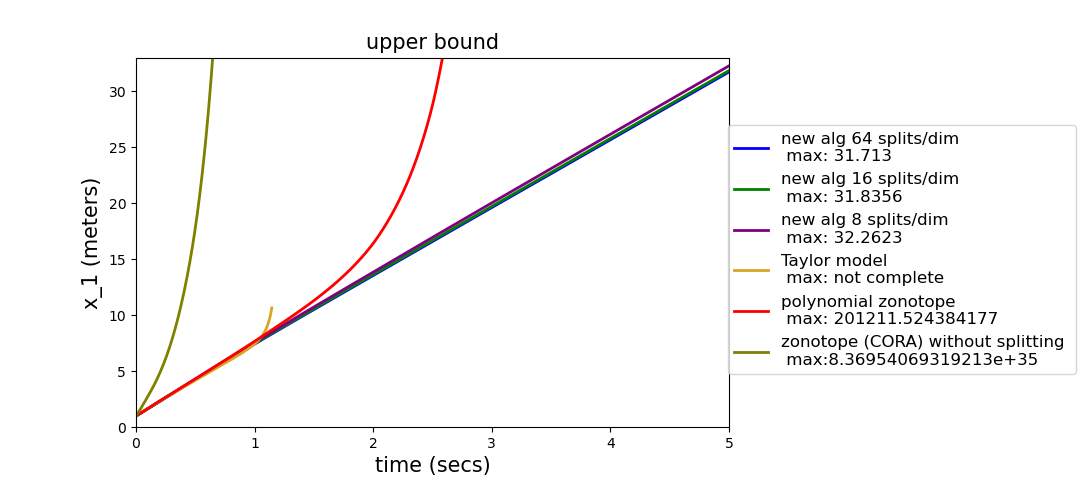
\includegraphics[width=6.4cm,height=4.8cm]{autocarImages/ubToolx1.png}%\hspace{-2.2em}
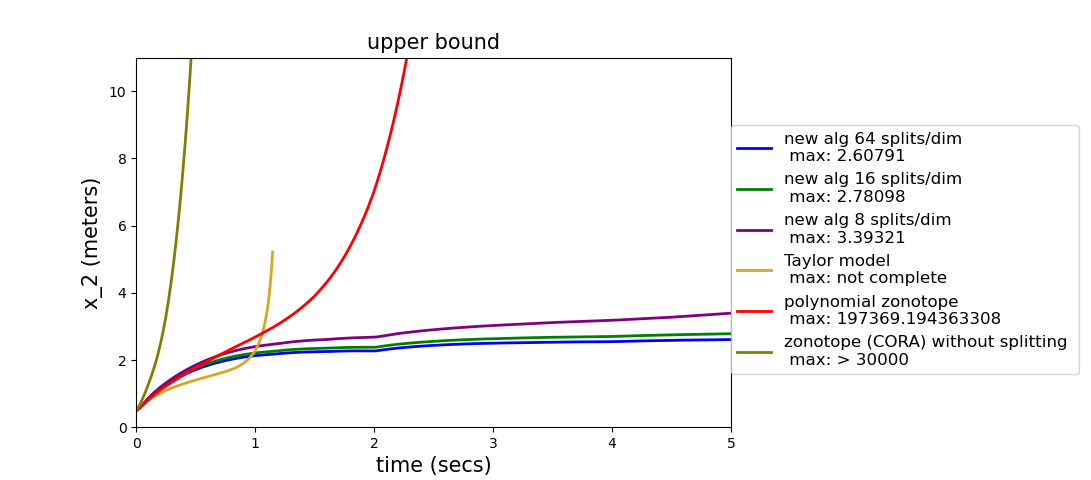
\includegraphics[width=6.4cm,height=4.8cm]{autocarImages/ubToolx2.png}
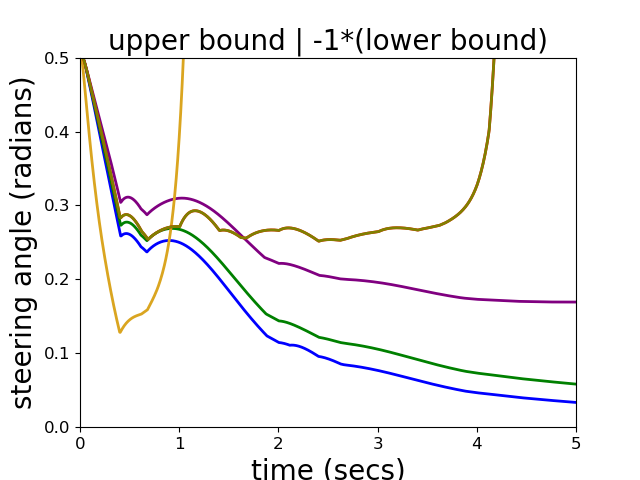
\includegraphics[width=6.4cm,height=4.8cm]{autocarImages/ubToolSteering.png}%\hspace{-2.2em}
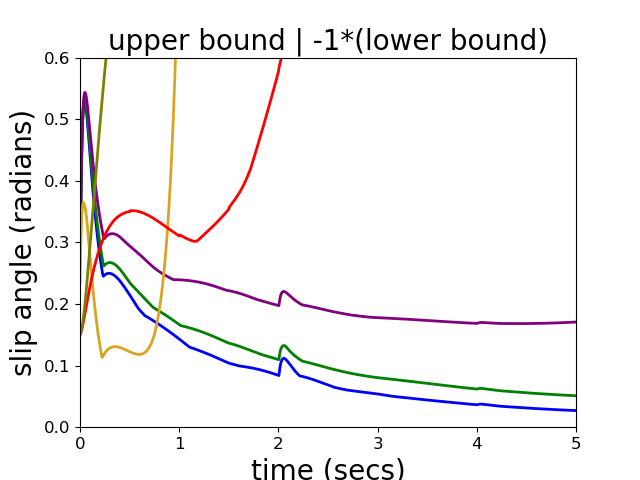
\includegraphics[width=6.4cm,height=4.8cm]{autocarImages/ubToolSlip.png}
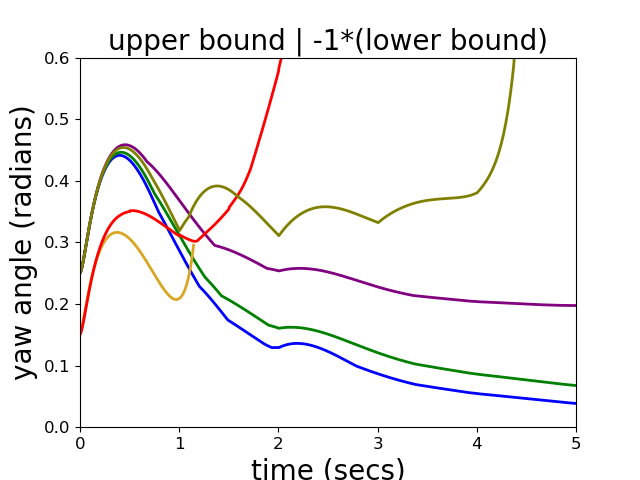
\includegraphics[width=6.4cm,height=4.8cm]{autocarImages/ubToolYaw.png}%\hspace{-2.2em}
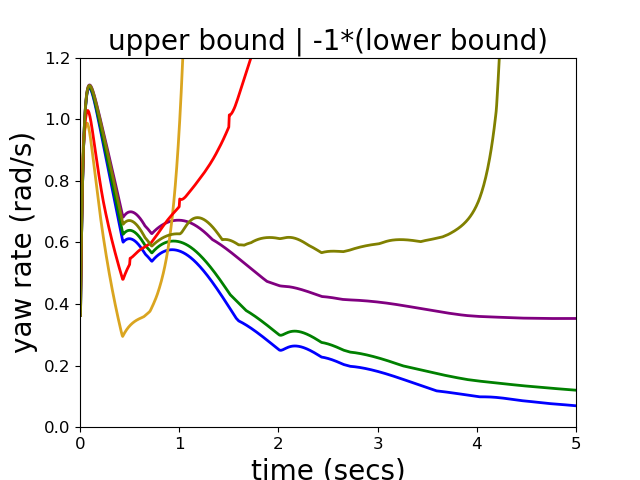
\includegraphics[width=6.4cm,height=4.8cm]{autocarImages/ubToolYawRate.png}


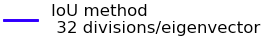
\includegraphics[scale = 0.39]{autocarImages/leg1.png}~
  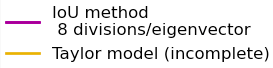
\includegraphics[scale = 0.41]{autocarImages/leg2.png}~
  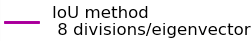
\includegraphics[scale = 0.41]{autocarImages/leg3.png}
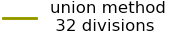
\includegraphics[scale = 0.39]{autocarImages/leg6.png}~
  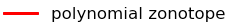
\includegraphics[scale = 0.41]{autocarImages/leg5.png}~
  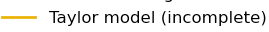
\includegraphics[scale = 0.41]{autocarImages/leg4.png}
  \caption{Flowpipe bounds at different time points for
    car model }\label{fig:flowcar}
\end{figure}
% \begin{figure}
% 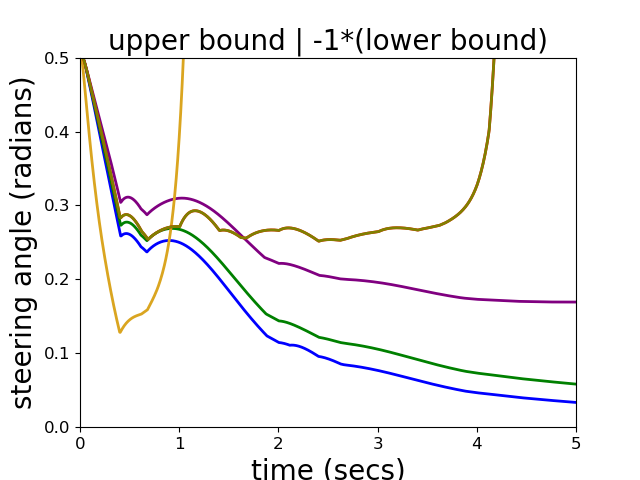
\includegraphics[scale = 0.39]{autocarImages/ubToolSteering.png}%\hspace{-2.2em}
% 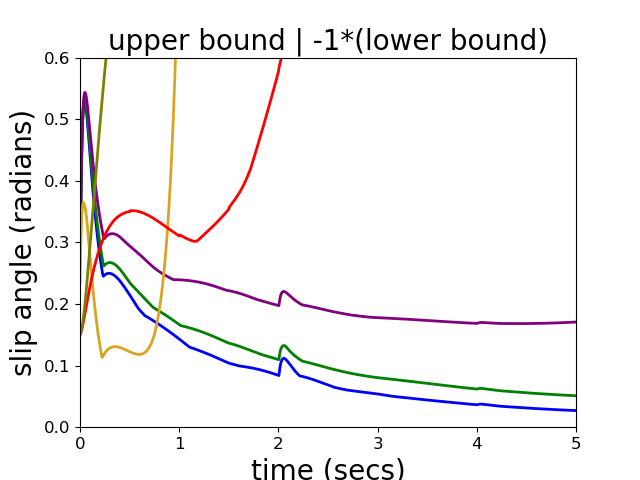
\includegraphics[scale = 0.39]{autocarImages/ubToolSlip.png}
% 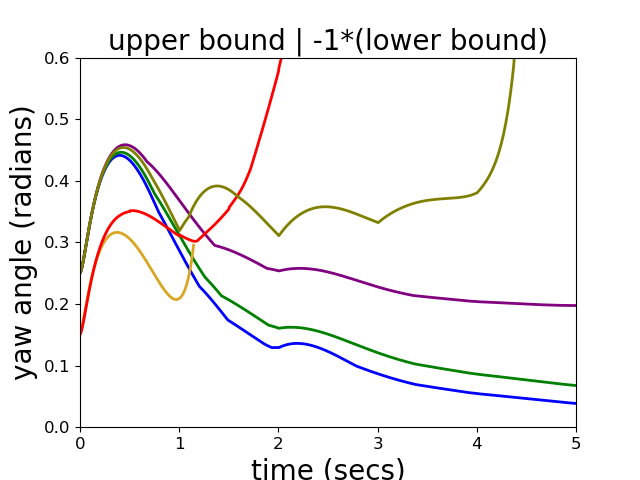
\includegraphics[scale = 0.39]{autocarImages/ubToolYaw.png}%\hspace{-2.2em}
% 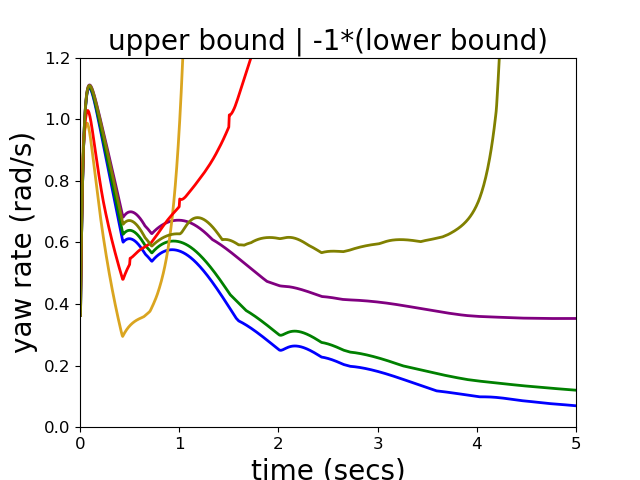
\includegraphics[scale = 0.39]{autocarImages/ubToolYawRate.png}
% 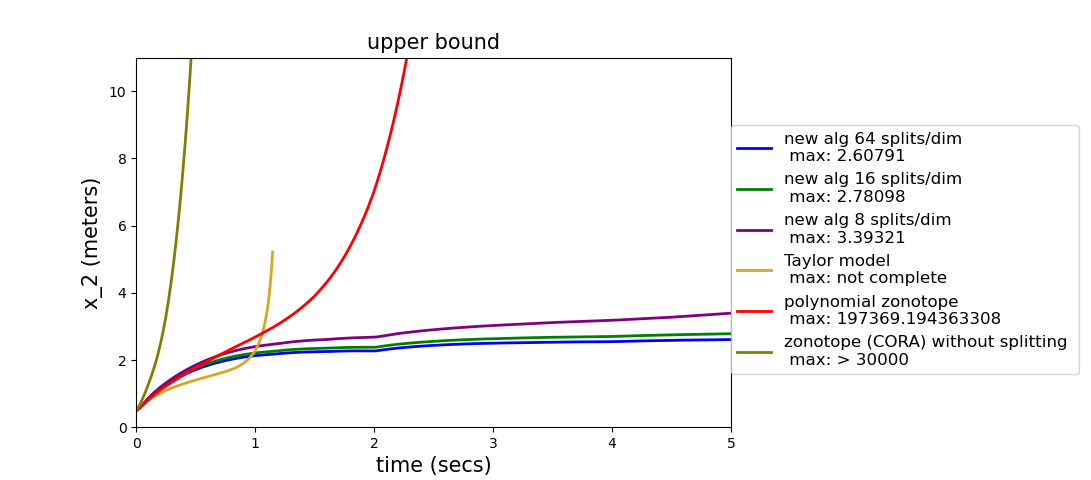
\includegraphics[scale = 0.41]{autocarImages/ubToolx2.png}%\hspace{-2.2em}
% 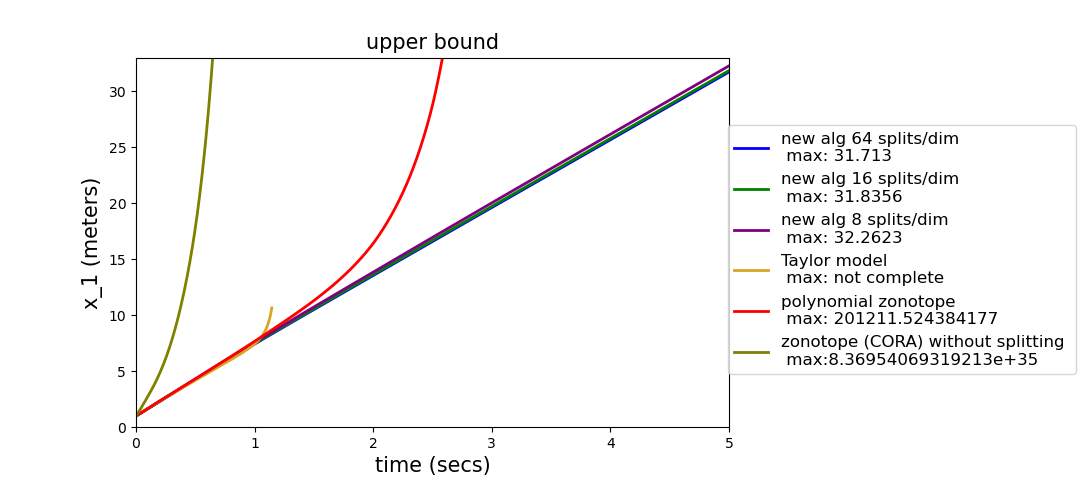
\includegraphics[scale = 0.39]{autocarImages/ubToolx1.png}

% 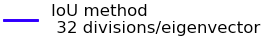
\includegraphics[scale = 0.39]{autocarImages/leg1.png}~
%   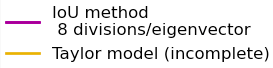
\includegraphics[scale = 0.41]{autocarImages/leg2.png}~
%   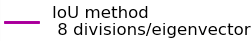
\includegraphics[scale = 0.41]{autocarImages/leg3.png}
%   \caption{Flowpipe bounds at different time points for
%     car model}\label{fig:flowcar}
% \end{figure}
%
\subsection{$7$-dimensional model of autonomous car}
\is{It may be good to emphasize on the tight coupling among the variables.}
A time discretized model of autonomous car manoeuvre with $7$-dimensional
state space and $2$ inputs was presented in~\cite{lavaei2020formal}.
We adapted this model into a continuous time system and provided a
stabilizing feedback with one of the inputs.  Then we have the
following $7$-dimensional system having only one
uncontrolled input.
%
\begin{align*}
\dot{x_1}  = & x_4\cos\rb{x_5+x_7}\hspace{2em} \dot{x_2} =
x_4\sin\rb{x_5+x_7}\\
%
\dot{x_3}  = & -r(x_5+x_7+x_3) \hspace{2em} \dot{x_4} =
 u \hspace{2em} \dot{x_5} = x_6 & \\
 %
 \dot{x_6}  = & \frac{\mu
 m}{I_z(l_r+l_f)}(l_fC_{Sf}(gl_r-uh_{cg})x_3+
 (l_rC_{Sr}(gl_f+uh_{cg})\\& -l_fC_{Sf}(gl_r-uh_{cg}))x_7
 -(l_fl_fC_{Sf}(gl_r-uh_{cg}) + l_rl_rC_{Sr}(gl_f+uh_{cg}))\frac{x_6}{x_4})\\
%
\dot{x_7} 
= & \frac{\mu}{x_4(l_r+l_f)}(C_{Sf}(gl_r-uh_{cg})x_3+(C_{Sr}(gl_f+uh_{cg})-C_{Sf}(gl_r-uh_{cg}))x_7\\
&-(l_f*C_{Sf}(gl_r-uh_{cg}) + l_rC_{Sr}(gl_f+uh_{cg}))x_6/x_4)-x_6
\end{align*}
%
Above, $x = \rb{x_1,\ldots,x_7}^T$ represents the state vector and $u$
is the input, while rest are constant parameters.  The 2-D position of
car is $(x_1,x_2)$, steering angle is $x_3$, heading velocity is
$x_4$, yaw angle is $x_5$, yaw rate is $x_6$ and slip angle is $x_7$.
The parameter values in S.I. units is 
%
$ g = 9.81, m = 1093.3, \mu = 1.0489, l_f = 1.156, l_r = 1.422, h_{cg}
  = 0.574, I_z = 1791.6, C_{Sf} = 20.89, C_{Sr} = 20.89, r = 4$.  We
  consider the input set $u\in U = [-0.01,0.01]$ and the initial set
  $X_0 =
  [-1,1]\times[-0.5,0.5]\times[-0.5,0.5]\times[5,6]\times[-0.25,0.25]\times[-0.2,0.2]\times[-0.25,0.25]$.
  We compare our IoU method with the union
  method~(Equation~\ref{eqn:pi}) and also Taylor models in Flowstar
  with high expansion order and polynomial zonotopes in CORA with
  large number of generators and dependent generators.

%% \emph{Settings:}  The simulation time step is $\delta = 0.005\si{\second}$.  
%% For the Flowstar Taylor model, the order of Taylor expansion is $9$.  
%% For the CORA polynomial zonotope, the generator order is $400$ and the order of dependent generators is $2000$.  
%% The zonotope order of our IoU method and the union method is $l=400$.  
%% Also, $K = 20$ and $\epsilon = 10^{-12}$.  
%% For the only union method, the normalization error
%%   error $\rho$ for division is the Taylor error before division
%%   $\taylor{f}{X_0}{u}$.  We ran our IoU method and the union method on
%%   an AWS c5a.16xlarge cluster with 64 virtual cpus.  For Flowstar, we
%%   used AWS t2.large instance.  We ran CORA in MATLAB 2019a on the
%%   computer specified in the previous illustrative example.

\emph{Results:}  The upper and lower bounds of flowpipe for different
  methods is plotted over uniformly space time stamps in
  Figure~\ref{fig:flowcar}.  There is very small change in the heading
  velocity, so it is not plotted.  Flowstar could not complete the
  Taylor model flowpipe simulation beyond $1.15\si{\second}$ due to
  large time discretization error.  The bottom 3 lines in the figure
  correspond to our IoU flowpipe method, which show convergence while
  all other plots are diverging.  The figure clearly shows a high
  increase in accuracy by using intersection of unions compared to
  other methods.  The simulation times are given in
  Table~\ref{tab:comptimes}.  The preprocessing time before simulation
  for IoU method is $18\si{\second}$, when the symbolic
  derivative and double derivatives of the vector field are computed and the C++ code is
  compiled.
  %
 %
\begin{table}
\begin{center}
\caption{Computation times}\label{tab:comptimes}
\begin{tabular}{|l|c|c|c|c|c|c|}
\hline
Example & IoU  & IoU  & IoU  & Only Union &
Polynomial & Taylor\\
& $\eta = 3$ & $\eta = 4$ & $\eta = 5$ & $\eta = 5$ & Zonotope & Model \\
\hline
& & & & & & {\color{red}Incomplete}\\
Car & 108 s & 128 s & 252 s & 122 s & 4068 s & {\color{red}[0,1.15s]:~216s}\\
\hline
& & & & & & {\color{red}Incomplete}\\
Quadrotor & 169 s & 318 s & 614 s & {\color{red}
Incomplete} & 2382 s & {\color{red}[0,4.13s]:~583 s} \\
\hline
\end{tabular}
\end{center}
\end{table}
%
\begin{figure}
%\vspace{-1.05em}
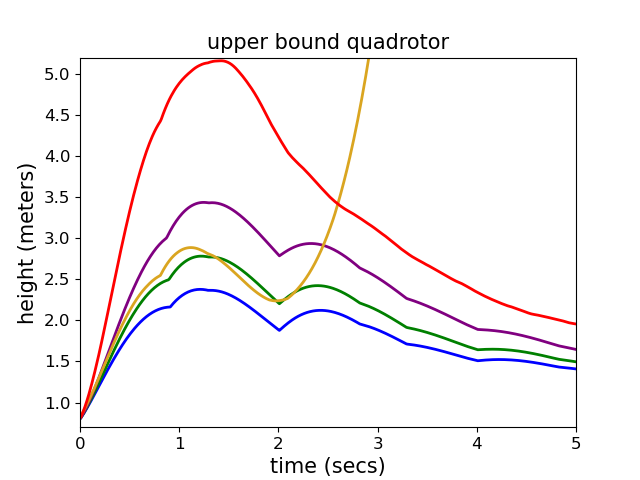
\includegraphics[width=6.4cm,height=4.8cm]{quadrotorImages/ubToolHeight.png}%\hspace{-2.2em}
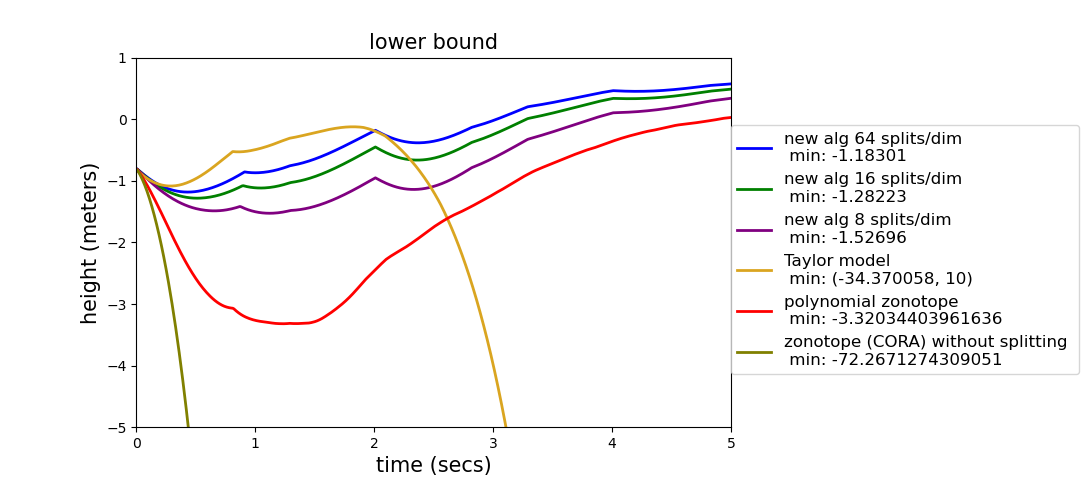
\includegraphics[width=6.4cm,height=4.8cm]{quadrotorImages/lbToolHeight.png}

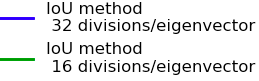
\includegraphics[scale = 0.41]{quadrotorImages/leg1.png}~
  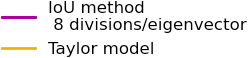
\includegraphics[scale = 0.41]{quadrotorImages/leg2.png}~
  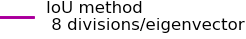
\includegraphics[scale = 0.41]{quadrotorImages/leg3.png}
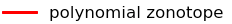
\includegraphics[scale = 0.41]{quadrotorImages/leg5.png}~
  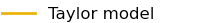
\includegraphics[scale = 0.41]{quadrotorImages/leg4.png}
\caption{Flowpipe bounds on height at different time points.
Note: Union method resulted in infinite bounds (not plotted).}\label{fig:flowquadrotor}
\end{figure}
% 
\subsection{$12$-dimensional model of quadrotor}
We consider the $12$-dimensional model of a quadrotor with three
inputs presented in the ARCH 2020 friendly
competition~\cite{geretti2020arch}, whose dynamics is given in the
appendix.  It has a $12$-dimensional state vector $x
= \rb{p_n,p_e,h,u,v,w,\phi,\theta,\psi,p,q,r}$, where $h$ is the
height of the quadrotor and a $3$-dimensional input vector $u
= \rb{u_1,u_2,u_2}$.  We take a larger initial set than the one given
in the competition~\cite{geretti2020arch} so that there is significant
linearization error in the flowpipe.  Our initial set in S.I. units
is $X_0 = [-0.8,0.8]^6\times[-0.5,0.5]^2\times[0,0]\times
[-1,1]^2\times[0,0]$.  The input set is $\rb{u_1,u_2,u_3}\in
[-0.99,1.01]\times[-0.01,0.01]^2$.  The goal of controller is to
stabilize the vertical height of the quadrotor at $h = 1\si{\meter}$.

%% \emph{Settings:}  The simulation time step is $\delta = 0.01\si{\second}$.  
%% For Flowstar Taylor model, the order of Taylor expansion is $7$.  For
%%   the CORA polynomial zonotope, generator order is $200$ and order of
%%   dependent generators is $2000$.  The zonotope order of our IoU
%%   method and the union method is $l=200$.  Also, $K = 20$ and
%%   $\epsilon = 10^{-12}$.  For the only union method, we take the
%%   normalization error $\rho$ as the Taylor error before division
%%   $\taylor{f}{X_0}{u}$.  We ran our IoU method and the union method on
%%   an AWS c5a.16xlarge cluster with 64 virtual cpus.  For Flowstar, we
%%   used AWS t2.large instance.  We ran CORA in MATLAB 2019a on the
%%   computer specified in the previous illustrative example.  The
%%   simulation time horizon is $[0, 5 s]$.
  
%% \is{The setting is mostly the same as the previous examples. Could we create a subsection on experimental setup before the examples and put these details there?}

\emph{Results:}  Our IoU method for each of the $8$, $16$ and $32$ divisions per
  eigenvector direction showed much higher accuracy than other
  methods.  We plotted the flowpipe bounds for the height in
  Figure~\ref{fig:flowquadrotor}.  The figure clearly shows high
  increase in accuracy by using intersection of unions compared to
  other methods.  The union method based on division using
  Equation~\ref{eqn:pi} resulted in very high linearization error and
  consequently infinite bounds after $0.5\si{\second}$ simulation
  time.  The computation times are given in Table~\ref{tab:comptimes}.
  The preprocessing time before simulation for our IoU method is
  $44\si{\second}$, when the symbolic derivative and double
  derivatives of the vector field are computed and the C++ code is compiled.
%

\is{A separate subsection for computation time?}
%
\section{Conclusion}
Dividing reachable set to restrict the linearization error below a
threshold can become computationally intractable in high dimensional
spaces.  Alternatively, we can fix the number of pieces and then find
a good division of the reach set that minimizes the linearization
error.  However, the linearization error being multi-dimensional, the
required optimization is multi-objective which has no single best
solution.  We addressed this issue by using intersection of unions,
where each intersecting union corresponds to an optimized division for
one direction of linearization error.  Evaluation of this method on
real world examples showed high increase in accuracy compared to
state-of-the-art techniques and an earlier method of division that uses only unions instead of intersection of unions.

There is a large scope for improvement of our method.  The
intersection between interval zonotopes is not computed very
accurately in this algorithm.  If this is improved, we can get
further gain in accuracy.  Furthermore, we only divide the
reachable set in the initial time interval because iterative division
increases the number of pieces and the complexity of representing the
reachable sets.  Thus, we need to find a way of controlling the
complexity of set representation while making iterative division such
that the resulting abstraction error is small.  Furthermore, we
believe that a GPU implementation of our parallel algorithm,
instead of using multiple CPUs, will result in better scalability.







\bibliographystyle{plain}
\bibliography{ref}

\section{Appendix}
\begin{appendix}
\paragraph{Dynamics of quadrotor}
%
\begin{align*}
  \dot{p_n} & = u cos(\phi) cos(\theta) - v (cos(\phi)
  sin(\psi)-cos(\psi) sin(\phi) sin(\theta)) + \\ & w (sin(\phi) sin(\psi)+cos(\phi) cos(\psi) sin(\theta))\\
   \dot{p_e} & = v (cos(\phi) cos(\psi)+sin(\phi) sin(\psi)
  sin(\theta)) + u cos(\theta) sin(\psi) - \\ &w (cos(\psi) sin(\phi)-cos(\phi) sin(\psi) sin(\theta))  \\                          
   \dot{h} & = u sin(\theta) - w cos(\phi) cos(\theta)  - v cos(\theta) sin(\phi)\\
   \dot{u} & = r v - q w - g sin(\theta)\\
   \dot{v} & = p w - r u + g cos(\theta) sin(\phi)\\
   \dot{w} & = q u - p v + g cos(\phi) cos(\theta) - (m g - 10 (h - u_1) + 3 w)/m\\
   \dot{\phi} & = p + r cos(\phi) sin(\theta)/cos(\theta) + q sin(\phi) sin(\theta)/cos(\theta)\\
   \dot{\theta} & = q cos(\phi) - r sin(\phi)\\
   \dot{\psi} & = r cos(\phi)/cos(\theta) + q sin(\phi)/cos(\theta)\\
   \dot{p} & = (-(\phi - u_2) - p)/Jx + q r (Jy-Jz)/Jx\\
   \dot{q} & = (-(\theta - u_3) - q)/Jy + p r (Jx-Jz)/Jy\\
   \dot{r} & = 0/Jz + p q (Jx - Jy)/Jz\\
\end{align*}
%
\end{appendix}



\end{document}
